% ****** Start of file apssamp.tex ******
%
%   This file is part of the APS files in the REVTeX 4.2 distribution.
%   Version 4.2a of REVTeX, December 2014
%
%   Copyright (c) 2014 The American Physical Society.
%
%   See the REVTeX 4 README file for restrictions and more information.
%
% TeX'ing this file requires that you have AMS-LaTeX 2.0 installed
% as well as the rest of the prerequisites for REVTeX 4.2
%
% See the REVTeX 4 README file
% It also requires running BibTeX. The commands are as follows:
%
%  1)  latex apssamp.tex
%  2)  bibtex apssamp
%  3)  latex apssamp.tex
%  4)  latex apssamp.tex
%
\documentclass[%
reprint,
superscriptaddress,
%groupedaddress,
%unsortedaddress,
%runinaddress,
%frontmatterverbose, 
%preprint,
%preprintnumbers,
%nofootinbib,
%nobibnotes,
%bibnotes,
amsmath,amssymb,
aps,
%pra,
prb,
%rmp,
%prstab,
%prstper,
%floatfix,
showkeys,
]{revtex4-2}
\usepackage[T1]{fontenc}
\usepackage{bera}
\usepackage{soul}

\usepackage{todonotes}
\usepackage{graphicx}% Include figure files
\usepackage{dcolumn}% Align table columns on decimal point
\usepackage{bm}% bold math
\usepackage{physics}
\usepackage{natbib}
\usepackage{epsfig}
\usepackage{epstopdf}
%\usepackage{dsfont}

\usepackage{hyperref}
%\usepackage[usenames,dvipsnames]{xcolor}
%\hypersetup{colorlinks, linkcolor={red},citecolor={blue}, urlcolor={MidnightBlue}}

%\usepackage{hyperref}% add hypertext capabilities
%\usepackage[mathlines]{lineno}% Enable numbering of text and display math
%\linenumbers\relax % Commence numbering lines

%\usepackage[showframe,%Uncomment any one of the following lines to test 
%%scale=0.7, marginratio={1:1, 2:3}, ignoreall,% default settings
%%text={7in,10in},centering,
%%margin=1.5in,
%%total={6.5in,8.75in}, top=1.2in, left=0.9in, includefoot,
%%height=10in,a5paper,hmargin={3cm,0.8in},
%]{geometry}

\begin{document}
	
	\preprint{APS/123-QED}
	
	\title{Dynamical Many Body Localization in Periodically Driven Long-Range Spin Systems: An Eccentric Phase Crossover}% Force line breaks with \\
	%\thanks{A footnote to the article title}%
	
	\author{Mahbub Rahaman}
	\affiliation{Department of Physics, The University of Burdwan, Golapbag, Bardhaman - 713 104, India}
	\author{Takashi Mori}
	\affiliation{RIKEN CEMS, 2-1 Hirosawa, Wako, Saitama, 351-0198, Japan}
	\author{Analabha Roy}
	\affiliation{Department of Physics, The University of Burdwan, Golapbag, Bardhaman - 713 104, India}
	
	\begin{abstract}
		The phenomenon of many-body localization occurs in quantum systems under specific resonance conditions, preventing thermalization and allowing the system to maintain its initial state. Quantum dynamical localization has been validated for multi-body spin systems under the influence of transverse field. The validation has been parameterized by the Inverse Participation ratio (IPR) of Floquet modes. Power-law dependence with long-range. The study applied $J_{ij} = 1/|i-j|^{\beta}$ and examined the short-range Transverse Field Ising Model for $\beta = \infty$ and the long-range Lipkin Meshkov-Glick (LMG) model for $\beta = 0$ at varying drive frequencies. The Ising model displays complete localization at high frequencies, while localization persists at low frequencies at the localization point. At the resonance point of system localization, LMG exhibits high-frequency localization in the long-range scenario. However, at lower frequencies, localization deteriorates following an inverse system size law. Chaos and regularity alternate at different frequencies in LMG at the phase-space continuum limit.IPR for LMG is evolved by an adiabatic increase in drive frequencies; the IPR rises gradually uotp unity  thereby manifesting a phase crossover which proposes a future protocol for the MBL engine.
		
		%\begin{description}
		%\item[Usage]
		%Secondary publications and information retrieval purposes.
		%\item[Structure]
		%You may use the \texttt{description} environment to structure your %abstract;
		%use the optional argument of the \verb+\item+ command to give the %category of each item. 
		%\end{description}
	\end{abstract}
	
	\keywords{Dynamical localization, Thermalization, Phase Crossover}%Use showkeys class option if keyword
	%display desired
	\maketitle
	
	%\tableofcontents
	
	Periodically driven Quantum Many Body Systems can experience Dynamical Freezing (DMF) when  dynamical hysteresis stops observables from reaching their diagonal averaged values and thermalizing to infinite temperature ~\cite{bordia_periodically_2017, sahoo_periodically_2019, das_exotic_2010}. Under certain resonance conditions in the drive parameters, DMF can cause the response to ‘freeze’ completely to its initial value at all times. This arises as a consequence of additional approximate symmetries that occur at resonance. DMF has been demonstrated via the Rotating Wave Approximation (RWA) in the driven TFIM with nearest neighbour interactions ~\cite{mbeng_quantum_2020} and is shown to be protected when translational invariance is explicitly broken (say, by disorder) ~\cite{yamada_localization_2022, roy_fate_2015}. 

	The utilization of Floquet theory simplifies the analysis of time-periodic systems. For closed quantum systems governed by the time-dependent Schr\"odinger equation, the \textit{Floquet Hamiltonian} allows for a mapping 
of the time-dependent dynamics into the dynamics of 	
a time-independent effective Hamiltonian, provided the system is strobed at integer multiples of the time period of the drive. The time independent eigenstates of the effective Hamiltonian correspond to quasi-stationary \textit{Floquet Modes} of the original Hamiltonian. The temporal progression of the system comes from  phase coefficients that capture the dynamics \cite{li_floquet_2018,eckardt_high_frequency_2015}.	
	
	Any sufficiently complex non-integrable Many Body System is expected to thermalize according to the Eigenstate Thermalization Hypothesis (ETH) despite the fact that closed quantum dynamics preserves the memory of the initial state of the system. This arises due to the properties of the matrix elements of observables 
	in typical states\cite{zhang_floquet_2016}. The ETH can be readily adapted to time-periodic systems using Floquet theory (the Floquet-ETH, or FETH). Nonetheless, the conditions for ETH to hold are not particularly strong, and the density matrix of the system can fail to approach one that is described by a thermal expression. In such cases, the system is said to undergo \textit{Many Body Localization} (MBL)\cite{khemani_phase_2016}. This phenomenon is stable against local perturbations, and constitutes an exotic state of matter with far-reaching implications in theoretical physics, as well as in practical applications\cite{yunger_halpern_quantum_2019}.
	
	The addition of disorder has been identified as a crucial component in the onset of MBL. In that case, thermalization is prevented by disorder-induced localization. An alternative approach to realizing MBL in clean many-body system involves \textit{Floquet Engineering}, where a time-periodic drive is introduced, and the drive parameters tuned so as to introduce a clustering of quasistationary energies in a manner similar to localization\cite{zhang_floquet_2016}.
	

	
	In this article, we propose that additional approximate symmetries can be Floquet-engineered in quantum many body systems with lower symmetry than the TFIM, such as those with long-range interactions. This results in both DMF and MBL occurring simultaneously at resonant values of the drive parameters, and complete thermal behaviour at other values. This phenomenon is distinct from DMF in the TFIM, since clean TFIM systems, being integrable, never thermalize.
	
	
	To demonstrate the onset of MBL, we investigate the driven Lipkin-Meshkov-Glick (LMG) model, a long-range system that is a special case of the more general Curie-Weiss model, wherein the nearest-neighbour exchange in the TFIM is extended to longer ranges with a power law dependence, $J_{ij}\sim 1/|i-j|^\beta$  ~\cite{campa_statistical_2009, eisele_multiple_1988, canning_class_1992}. Setting $\beta=\infty$ recovers the TFIM, and setting $\beta=0$ yields the LMG model. We have recovered the onset of DMF in this system and have supported our result with numerical simulations.
	
	In addition, we compare the degree of localization of the quasi-stationary Floquet modes in both limits of $\beta$. In order to do so, we look at the Inverse Participation Ratio (IPR) of the Floquet modes in the representation given by the eigenstates of the symmetry-breaking field. The IPR, closely related to the concept of quantum purity, is defined as the formal sum of the square of the density in some physically meaningful space or representation. A high IPR of a stationary state denotes low participation in most of the representation, and a low IPR distributes participation uniformly across the representation, leading to ergodic dynamics\cite{vu_fermionic_2022}. Thus, IPR~\cite{Misguich2016} is a useful tool for witnessing MBL of a quantum system. For an MBL system, the IPR is unity, and it scales inversely with the system size when it is thermally distributed~\cite{calixto_inverse_2015}.
	
	In the first section of this paper, we present all essential theoretical frameworks. Our results for the LMG model are presented next in section II. In that section, we have used the Rotating Wave Approximation (RWA) ~\cite{fujii_introduction_2017}, where only the slowest rotating terms in the Fourier expansion of the Hamiltonian in a frame co-rotating with the symmetry breaking drive field are retained. In addition, we have the obtained analytical expressions for the Floquet modes and their IPR. They are used to probe the system dynamics in the high and low-frequency domains at both limits of $\beta$. In section III we have used phase space plots to contrast the low and high frequency limits of the LMG model in the thermodynamic limit by mapping it to an equivalent classical Hamiltonian system. Finally, in section IV, we have looked at numerical computations of the IPR of the Floquet modes for different values of the drive parameters, well beyond those that allow for the RWA. We observed that, if the system is driven by an adiabatically increasing drive frequency from low to high limit while remaining in the resonance region, a sharp crossover from a thermal to an MBL phase occurs. We conclude with discussions and outlook.
	
\section{\label{sec:background} Background}
	
The Eigenstate Thermalization Hypothesis (ETH) is a series of conjectures that allows for the thermalization of an isolated quantum many body system. The state of the system, $\ket{\psi(t)}$, evolves according to the Schr\"odinger equation $\hat{H}\ket{\psi(t)} = i\displaystyle\frac{\partial}{\partial t}\ket{\psi}$. The Hamiltonian $\hat{H}$ is assumed to be \textit{non-integrable}, in that it lacks an extensive number of \textit{local} additive conserved quantities, that is to say, there are no set of observables $\hat{O}_s$ such that $\hat{H}=\sum_s \hat{O}_s$ for any extensive index $s$. Here, the $\hat{O}_s$ constitute an arbitrary CSCO (complete set of commuting observables) that are \textit{local}, having sub-extensive support in the system size. In addition, we postulate the existence of an equivalent Hamiltonian $\hat{H}_{eq}$ for every Hamiltonian $\hat{H}$ as well as an "equilibrium" value $A_{eq}$ for every observable $\hat{A}$, such that
\begin{equation}
	\label{eq:aeq}
 A_{eq}(E)\equiv \frac{\Tr \left(\hat{A}e^{-\beta \hat{H}_{eq}}\right)}{\Tr(e^{-\beta \hat{H}_{eq}})}.
\end{equation}

where $E=\expval{\hat{H}}{\psi(t)}$ is the conserved energy of the system, and $\beta = 1/(k_B T)$ is the inverse temperature, $H_{eq}$ is an effective Hamiltonian that captures the long-time average dynamics of the system, and $k_B$ is the Boltzmann constant.

To put it simply, ETH proposes that this many-body Hamiltonian undergoes thermalization as seen in the \textit{long-time averages} of observables, with the eigenstates bearing resemblance to thermal states. The aforementioned hypothesis serves as a valuable instrument for comprehending the conduct of stimulated quantum systems and their correlation with thermal equilibrium. This assertion can be justified by examining the expectation value of an observable $\hat{A}$ as it evolves under the Schr\"odinger equation. To see this, we first expand the state of the system $\ket{\psi(t)}$ as:
\begin{equation*}
\ket{\psi(t)} =  \sum_m c_m(t)\ket{m(0)},\\ 
\end{equation*}
where $\ket{m(0)}$ represents the eigenstates of $\hat{H}(0)$ with energy $E_m$. The coefficients $c_m (t)$ describe the time-dependent amplitude of the expansion.
Plugging these expansions into the expression for the expectation value, we obtain the long-time average of the expectation value~\cite{abanin_colloquium_2019}:
\begin{equation}
	\overline{\expval{\hat{A}(t)}} 
	= \sum_{m,k} \overline{c_m^\ast(t) c_k(t)}
	\mel{m(0)}{\hat{A}}{k(0)},
\end{equation}
Had the system been integrable, the large number of conserved quantities would restrict mixing between the states during unitary evolution. In the non-integrable case,
the system explores the entire Hilbert space spanned by eigenstates with eigenvalues close to $E$ more-or-less uniformly. In that case, the matrix elements $\mel{m(0)}{\hat{A}}{k(0)}$ are said to satisfy the Srednicki ansatz~\cite{Srednicki1994,Srednicki_1999}:
\begin{multline}
	\mel{m(0)}{\hat{A}}{k(0)} \approx A_{eq} \delta_{mk} +\\ e^{-\frac12 S\left(\frac{E_m+E_k}{2}\right)} f\;\left(\frac{E_m+E_k}{2}, E_m-E_k\right)R_{mk}.
\end{multline}
Here, $S$ is the thermodynamic entropy and $R_{mk}$ are elements of a random matrix with vanishing mean and unit variance. What this means for the ensuing dynamics is that the system explores the accessible Hilbert space uniformly,  and the matrix elements $\bra{m(0)}\hat{A}(t)\ket{k(0)}$ become indistinguishable for most pairs of $m$ and $k$.
Applying this ansatz and taking the thermodynamic limit by ignoring terms $\mathcal{O}(e^{-S/2})$, the expression for the expectation value becomes:
\begin{equation*}
\overline{\expval{\hat{A}(t)}} \approx \sum_m \overline{\abs{c_m(t)}^2} {A}_{eq}= {A}_{eq},
\end{equation*}

Therefore, in the limit of large systems the expectation value of an observable $\hat{A}$ is approximately equal to the thermal expectation value $A_{eq}$. This is the essence of the ETH, which suggests that individual eigenstates of a quantum system can be described by statistical mechanics in the long-time limit.

We now generalize the ETH to non-integrable many body systems that are closed, but not isolated. In that case, it is possible to impart a periodic time-dependence on the Hamiltonian while still ensuring unitary evolution. If the time period of the drive is $T$, and the corresponding drive frequency $\omega\equiv 2\pi/T$, the Floquet theorem states that the solutions to the Schrödinger equation can be written as $\ket{\psi(t)} = e^{-i\epsilon t/\hbar} \ket{\phi(t)}$, where the $\ket{\phi(t)}$ are $T$-periodic states called \textit{Floquet Modes}, the corresponding $\epsilon\in \mathbb{R}$, are called \textit{quasienergies}. Quasienergy values are not unique, and can be made to be bounded within a Floquet photon,\textit{viz.} a range $[-\omega/2, \omega/2]$\cite{holthaus_floquet_2016,vogl_effective_2020}. As a consequence, the unitary evolution operator can be spit into two parts as follows~\cite{Bukov2014}.
\begin{equation}
	U(t) = e^{-i\hat{K}_F(t)}\;e^{-i\hat{H}_Ft}.
\end{equation}
Here, the micromotion operator $\hat{K}_F(t)$ is time-periodic in $T$, with $\hat{K}_F(0)=0$, and the Floquet Hamiltonian $\hat{H}_F = \hat{H}(t) - i \displaystyle\frac{\partial}{\partial t}\bigg\vert_{t=T}$. Thus, if the system is strobed at integer multiples of $T$ only, then the unitary evolution matches that of a time independent Hamiltonian $H_F$. This can capture a representative cross-section of the exact dynamics at large frequencies.

In such systems, the Floquet Eigenstate Thermalization Hypothesis (FETH) posits that subject to specific conditions and in the context of a system of significant size, the Floquet modes themselves exhibit thermal state-like behavior, \textit{i.e.}, $\hat{H}_{eq}\approx \hat{H}_F$ in eqn~\ref{eq:aeq}. However, in contrast to the isolated systems, the loss of energy conservation allows for the mixing of all Floquet modes in the ensuing dynamics, not just those with quasienergies near $E$. Were this to actually happen in the ensuing dynamics, it can be reconciled with ETH~\cite{alessio} by ensuring that $\beta=0$ in eq~\ref{eq:aeq}. In other words, the nonequilibrium steady state of the system tends to an infinite temperature, maximum entropy density matrix.

However, drive parameters like amplitude, frequency, and duty-cycle strongly affect the structure of the Floquet modes $\ket{\phi}$. Thus, they can be engineered to prevent the kind of full mixing that would lead to infinite temperatures, manifesting suppression of thermalization dynamically. Thus, this type of \textit{Floquet Engineering} can produce \textit{Dynamical Many Body Localization} (DMBL), where the system fails to reach thermal equilibrium and remains localised, possibly  near its initial state, even at large times. This paradigm seems similar to standard Many-Body Localization\cite{yousefjani2023, sierant_2023}, where disorder, locality, and integrability can cause athermality via breakdown in the Srednicki ansatz. However, DMBL is a purely dynamical phenomenon, and thus can occur regardless of disorder, locality of observables, or system integrability, all of which have been studied for MBL onset~\cite{Sougata2023,Fabien2018,garratt_resonant_2022}.

Integrable Many Body systems do not exhibit thermalization. When subjected to time-periodic drives, Floquet engineering allows for the introduction of additional approximate conserved quantities that dynamically suppress the evolution of certain observables by hysteresis. This type of \textit{freezing} of response
has been shown in integrable systems~\cite{roy_fate_2015}.
A paradigmatic example is  the driven Transverse Field Ising model (TFIM) in one dimension~\cite{stinchcombe_ising_1973}. The Hamiltonian is given by
	\begin{align}
		\label{eq:tfim:hamilt}
		\hat{H}(t) &= \hat{H}_0 + h_z(t) \; \hat{H}_1\\
		\hat{H}_0 &= -\frac{1}{2}\sum^N_{i=1} \sigma^x_i \sigma^x_{i+1}\\
		\hat{H}_1 &= -\frac{1}{2}\sum_{i=1}^N \sigma^z_{i}.
	\end{align}
Here, the undriven Hamiltonian $\hat{H}_0$ consists of nearest-neighbour interactions between $N$ number of  spin-$1/2$ particles on a one-dimensional spin network. The transverse field is denoted by $\hat{H}_1$, and is being varied by a time-periodic and harmonic signal $h_z(t) = h_0 + h\cos{\omega t}$, yielding a time period $T=2\pi/\omega$ with amplitude $h$, drive frequency $\omega$, and d.c. field $h_0$. This Hamiltonian can be readily transformed into a spinless pseudo-fermionic system via the Jordan-Wigner transformation ~\cite{mbeng_quantum_2020}. When written in momentum space spanned by spinors $\psi_k = (c_{-k}, c^\dagger_k)^T$ of fermions at momentum $k$ created (annihilated) by operators $c^\dagger_k$ ($c_k$), the effective Hamiltonian
	\begin{equation}
		H(t) = \sum_{(k,-k)-\mbox{pairs}} \psi^\dagger_k
		\Bigg[\ \bigg(f_k - h_z(t)\bigg)\tau_z +  \tau_x \Delta_k\Bigg]\psi_k
	\end{equation}
	with $f_k = J\cos{k}$, $\Delta_k = J\sin{k}$, $\tau_{xyz}$ are the three Pauli Matrices, and the sum is over distinct $(k, -k)$ \textit{Cooper Pairs}. A transformation to the rotated frame is achieved by means of the unitary transformation operator $U(t) = \prod_k U_k(t)$, where $U_k(t) = \exp{\Big[\frac{i h}{\omega}\sin{\omega t}\Big]\tau_z}$. The resulting transformed Hamiltonian is 
	\begin{multline*}
		H^\prime(t) = \sum_{(k,-k)-\mbox{pairs}} \psi^\dagger_k
		\bigg[\ \tau_z f_k + \tau_x \cos{\big(\eta\sin{\omega t}\big)}  \\
		+ \tau_y \cos{\big(\eta\sin{\omega t}\big)}\bigg]\psi_k,
	\end{multline*}
	where we defined $\eta=2h/\omega$. Using the Jacobi-Anger formula~\cite{arfkenmath}
	\begin{equation}
		\label{eq:jacobi}
	e^{i \eta \sin{\omega t}} = \displaystyle\sum_{n=-\infty}^{\infty} J_n(\eta)\, e^{i n \omega t},
	\end{equation} 
	where $J_n(\eta)$ are Bessel Functions, the transformed Hamiltonian simplifies to \\
	\begin{align}
		H^\prime(t) =& \sum_{\substack{(k,-k) \\ \mbox{pairs}}} \psi^\dagger_k
		\bigg\{\ \tau_z f_k + 2\tau_x \Delta_k \sum_{n\geq 0} J_{2n}(\eta)\cos{\big(2n\omega t\big)} \nonumber\\
		&\hskip 0.7cm- 2\tau^y\Delta_k \sum_{n\geq 0} J_{2n+1}(\eta)\sin{\big[\left(2n+1\right)\omega t\big]}   \bigg\}\psi_k,
	\end{align}\\
	In the frequency regime  $\omega \gg f_k$, the long-time average $H^{RWA}\equiv\displaystyle\lim_{n\rightarrow\infty}\frac{1}{nT}\int^{nT}_0\mathrm{d}t\;H^\prime(t)$ can serve as a suitable approximation for $H^\prime(t)$. This approximation, known as the \emph{Rotated Wave Approximation} (RWA), eliminates the oscillating modes and results in an effective Hamiltonian that is independent of time.
	\begin{equation}
		\label{eq:hrwa:tfim}
		H^{RWA} = \sum_{(k,-k)-\mbox{pairs}} \psi^\dagger_k
		\bigg[\ f_k\tau_z + 2 J_0(\eta) \Delta_k\tau_x \bigg]\psi_k,
	\end{equation}
	It is evident that by manipulating the drive parameters, specifically the amplitude denoted by $h$ and the frequency denoted by $\omega$, in a manner such that $\eta$ is positioned on a root of $J_0(\eta)$, the fermion number can be conserved to a significant extent at this particular resonance. Consequently, it is feasible to exercise direct control over $H^{RWA}$, resulting in a comprehensive suppression of the dynamics of otherwise responsive observables. 
	
	This phenomenon is highly general in nature, and can be readily adapted to non-integrable systems. In such cases, freezing has the additional effect of inducing DMBL, suppressing thermalization to infinite temperatures. Numerical quantification of localization of a specific (quasi) stationary state in a physically significant representation can be achieved through the computation of the \emph{Inverse Participation Ratio} (IPR).  In the position representation, the IPR for a state $\ket{\psi}$  \cite{mukherjee_modulation-assisted_2015,lin_many-body_2018,murphy_generalized_2011, torres-herrera_self-averaging_2020} is defined as
	\begin{equation*}
		\phi_{IPR}\equiv \int \mathrm{d}\mathbf{x}\;\vert\ip{\mathbf{x}}{\psi}\vert^4
	\end{equation*}
	This definition can be generalized to the IPR of a state $|\phi\rangle$ in a representation given by complete orthonormal basis $\ket{m}$ as 
	\begin{equation}
	\label{eq:ipr:defn}
	\phi_{{_{IPR}}} \equiv \sum_m\vert\ip{m}{\psi}\vert^4.
	\end{equation}
	The smallest value of the IPR corresponds to a fully delocalized state, $\psi(x)=1/\sqrt{N}$ for a system of size $N$ \cite{torres-herrera_self-averaging_2020,trivedi_can_2005}. Values of the IPR close to unity correspond to localized states \cite{misguich_inverse_2016}. For a periodically driven system, we look at the IPR of the quasi-stationary Floquet modes at $t=T$, where $t=2\pi/\omega$ for drive frequency $\omega$. In the TFIM model, equation~\ref{eq:hrwa:tfim} indicates that, at resonance, when $J_0(\eta)=0$, the Floquet modes are approximately given by the fermionic Fock states, which have a trivially unit IPR in the representation of the eigenmodes of the transverse field $\hat{H}_1$ in equation~\ref{eq:tfim:hamilt}. Here, a particular Floquet mode can be decomposed into a direct product of cooper-pair states as $|\phi\rangle = \prod_{k,-k}|\phi^n_k\rangle$. In the RWA limit and at resonance, $|\phi^n_k\rangle$ has values of $|0\rangle, |k,-k\rangle$ for two values of $n=0,1$ respectively. We define the reduced IPR of $|\phi^n_k\rangle\; \forall k$ to be
	\begin{equation}
	\label{eq:ipr:ising}
	\phi^{(n)}_{IPR}(k) = \abs{\ip{0}{\phi^n_k}}^4 + \abs{\ip{ +k, -k }{\phi^n_k}}^4,
	\end{equation}
	where $n=0,1$. In the RWA limit and at resonance , this quantity is unity, indicating very low participation and the onset of freezing.
	\begin{figure}[hbt!]
		\centering
		%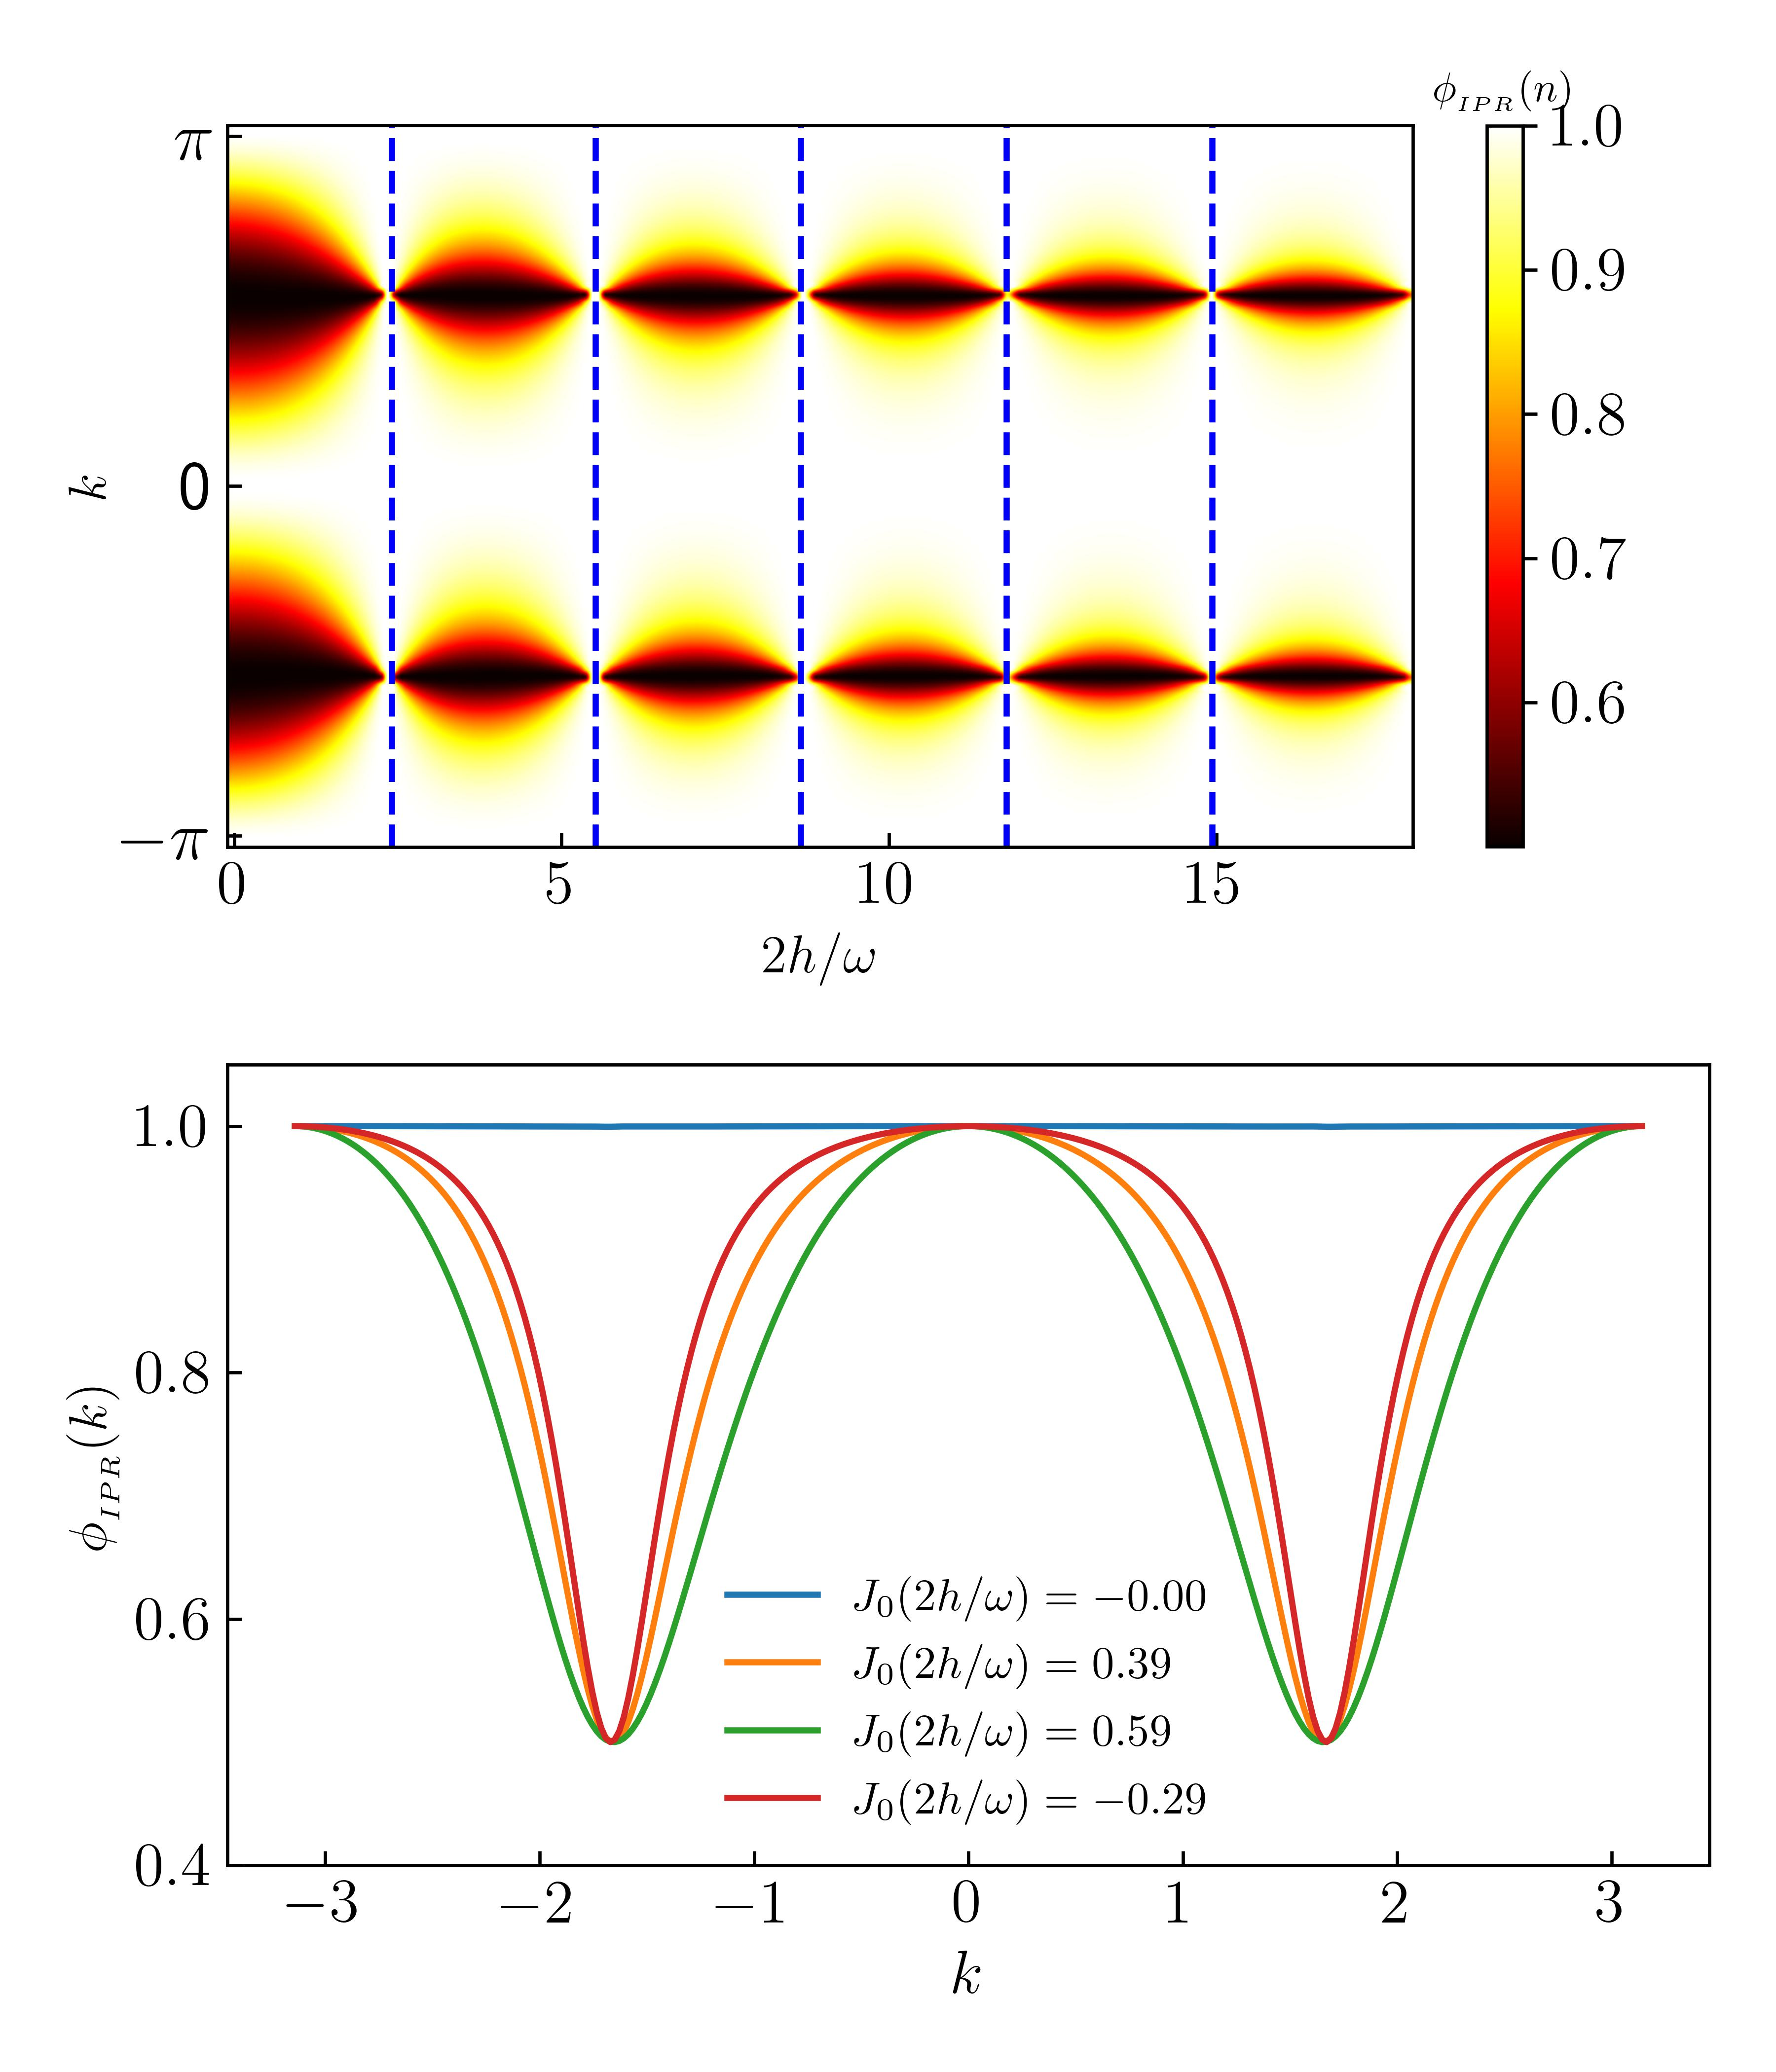
\includegraphics[height = 10cm, width = 9.0cm]{ising_exact_ipr.jpeg}
		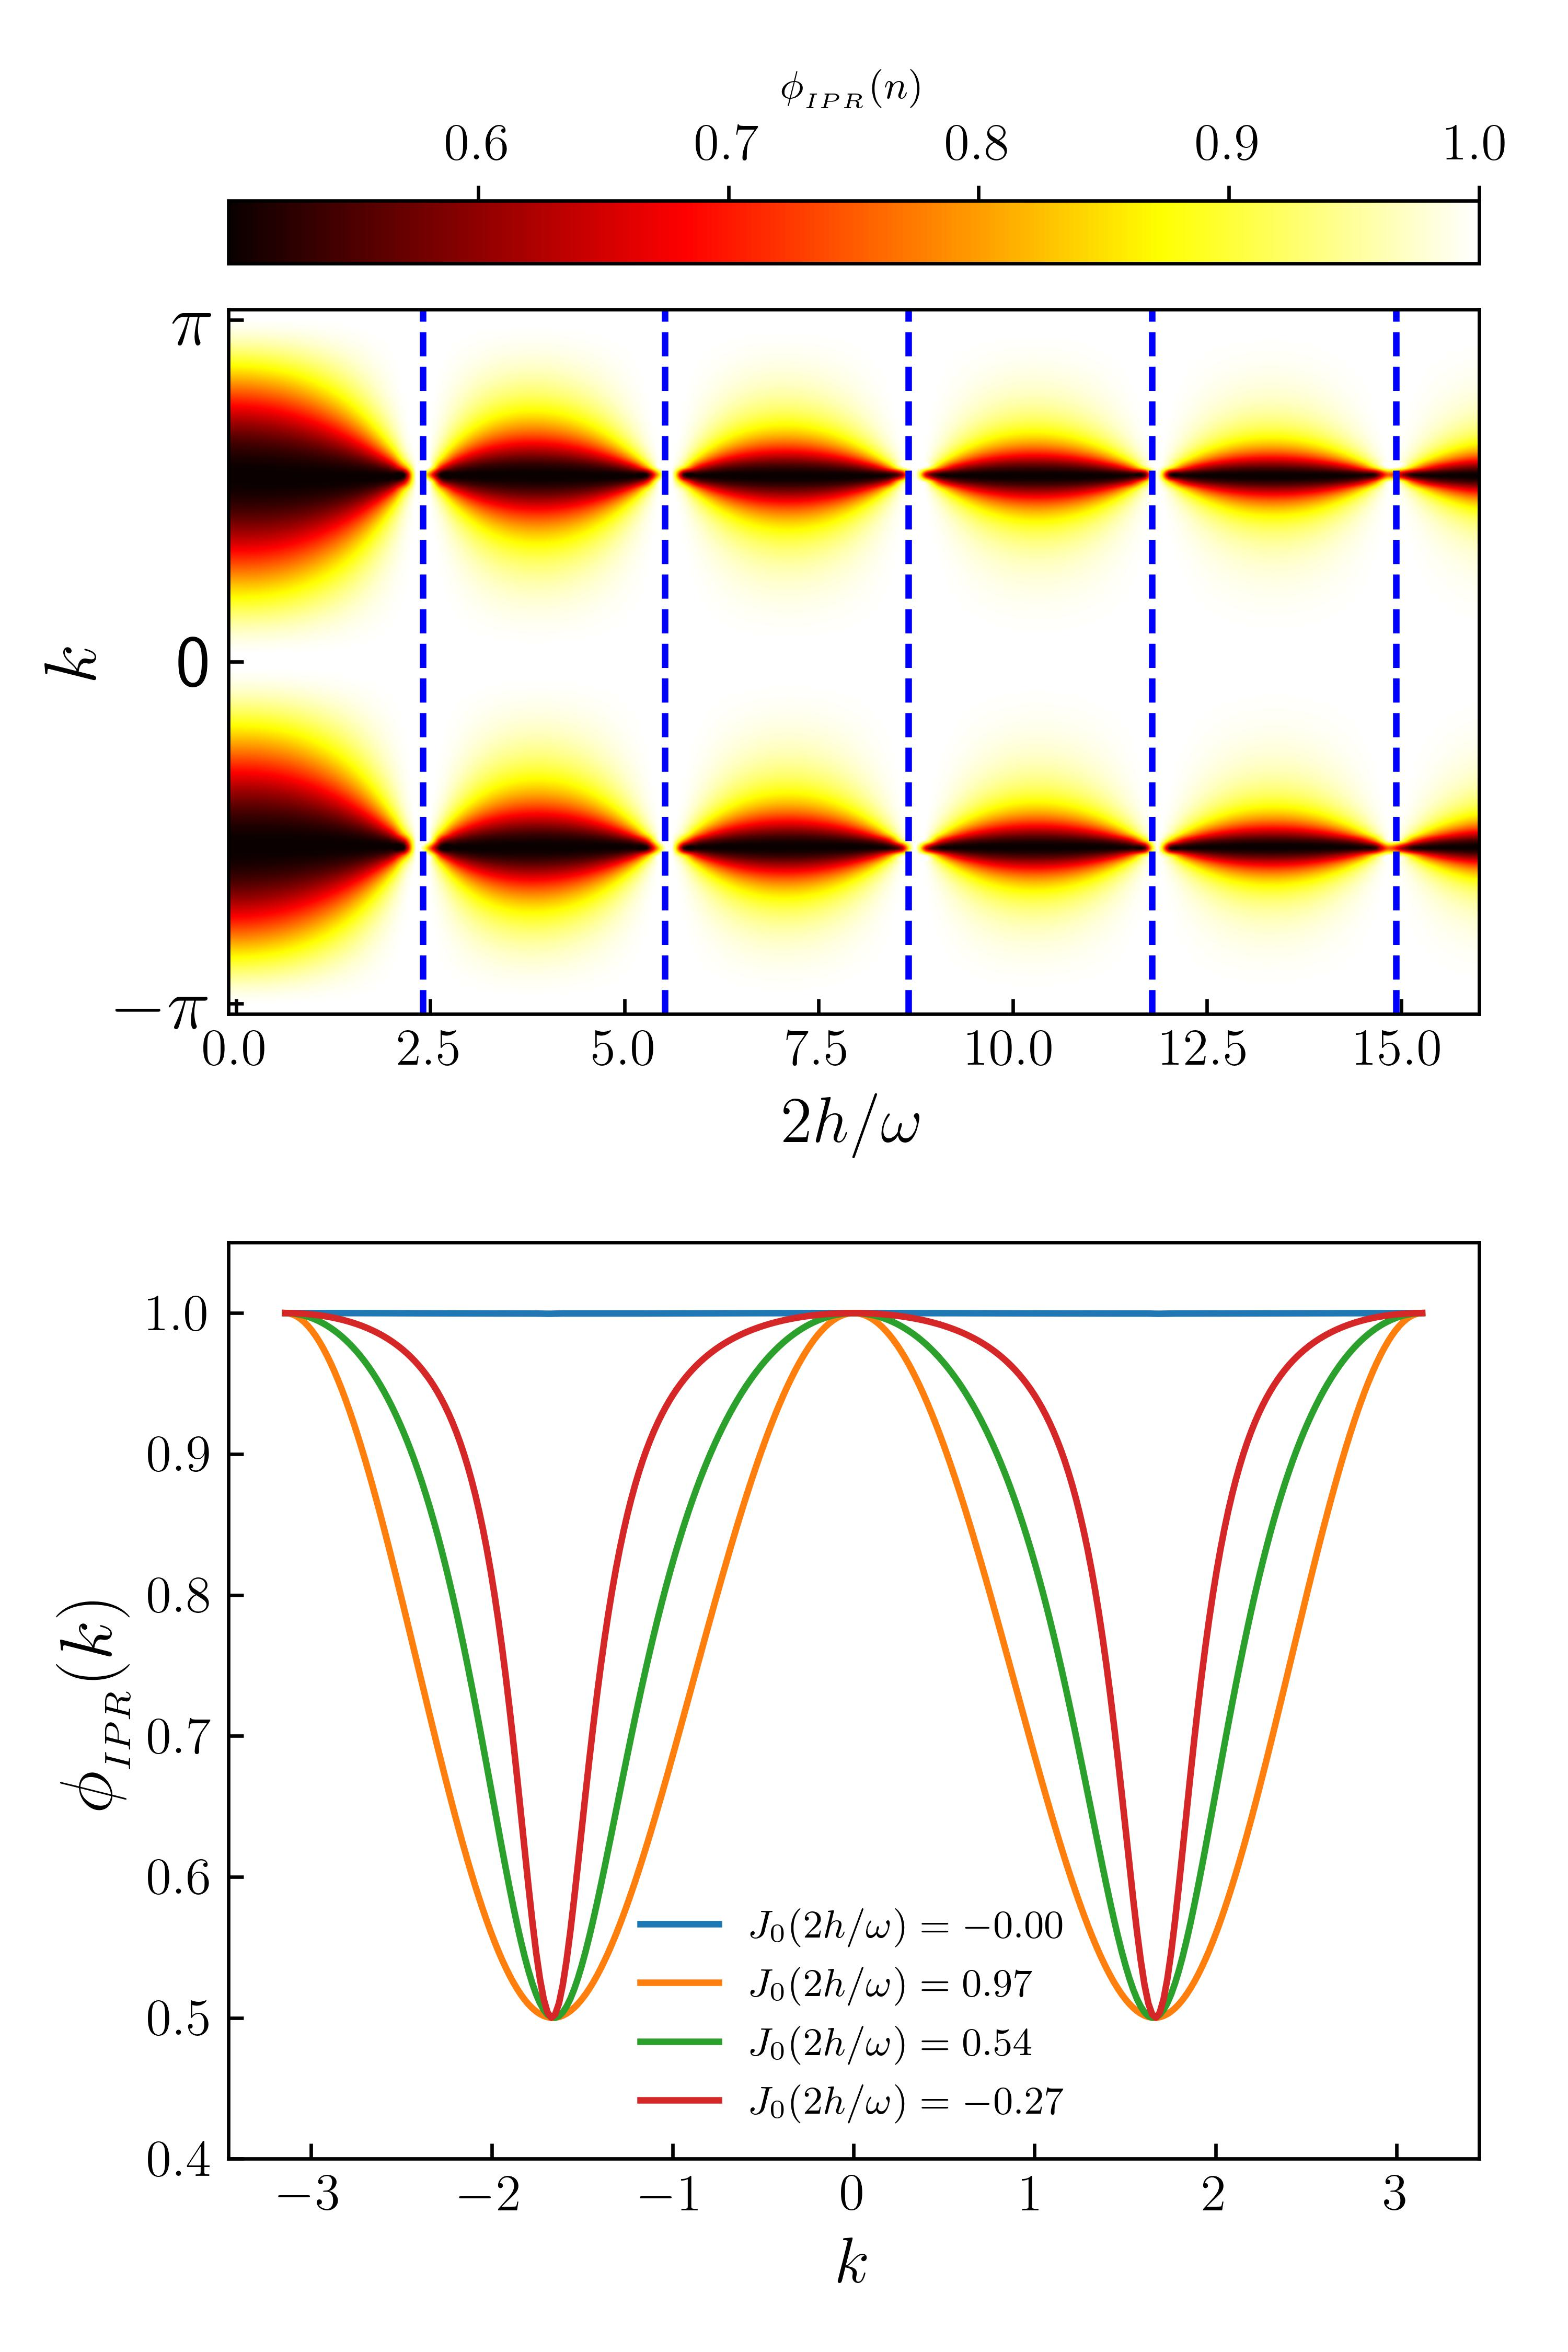
\includegraphics[width = 9.0cm]{ising_exact_ipr 1.jpeg}
		\caption{Reduced IPR (defined in equation~\ref{eq:ipr:ising}) for one of the two Floquet modes obtained from the
			exact dynamics of the TFIM for size $N = 100$ and $\omega=90$ for the entire Brillouin zone (top panel, ordinate) and a few drive amplitudes (top panel, abscissa). The dashed lines indicate the roots of $J_0(\eta)$.
			The bottom panel shows cross-sections for four different chosen amplitudes.}
		\label{fig:ipr:tfim}
	\end{figure}
	Figure~\ref{fig:ipr:tfim} shows results from numerically simulating the TFIM dynamics. The reduced IPR for a particular Floquet mode recovered by simulating the exact Schr\"odinger dynamics over a single time period of the drive, and plotted as a function of momentum $k$ for different $\eta$'s. At resonance, when $\eta$ lies at the root of the Bessel function $J_0(\eta)$,  the IPR is exactly unity for all momenta. Outside this resonance, the IPR is unity only for some momenta because the effective Hamiltonian is perfect diagonal at $k \in{\{-\pi, 0, \pi\}}$ as can be seen in the cross-sectional plots of figure~\ref{fig:ipr:tfim}. As we move away from the resonance point, IPR reduces from unity. However, as the TFIM is an integrable spin model, the IPR never drops to a value that is small enough to indicate thermalization. At low frequencies, RWA fails due to the unavailibity of zero off-diagonal terms in the  effective transformed Hamiltonian, as well as the absence of integrability breaking terms to counteract the off diagonal terms. Consequently,  the IPR remains quite high ($\sim 0.5$) even at the resonance point as can be seen figure~\ref{fig:ipr:isinglowfr}. At low frequency, this is valid for all momentum and parameter $\eta$, see figure~\ref{fig:ipr:isinglowfrk}.
	
	
	
	\begin{figure}[hbt!]
		\centering
		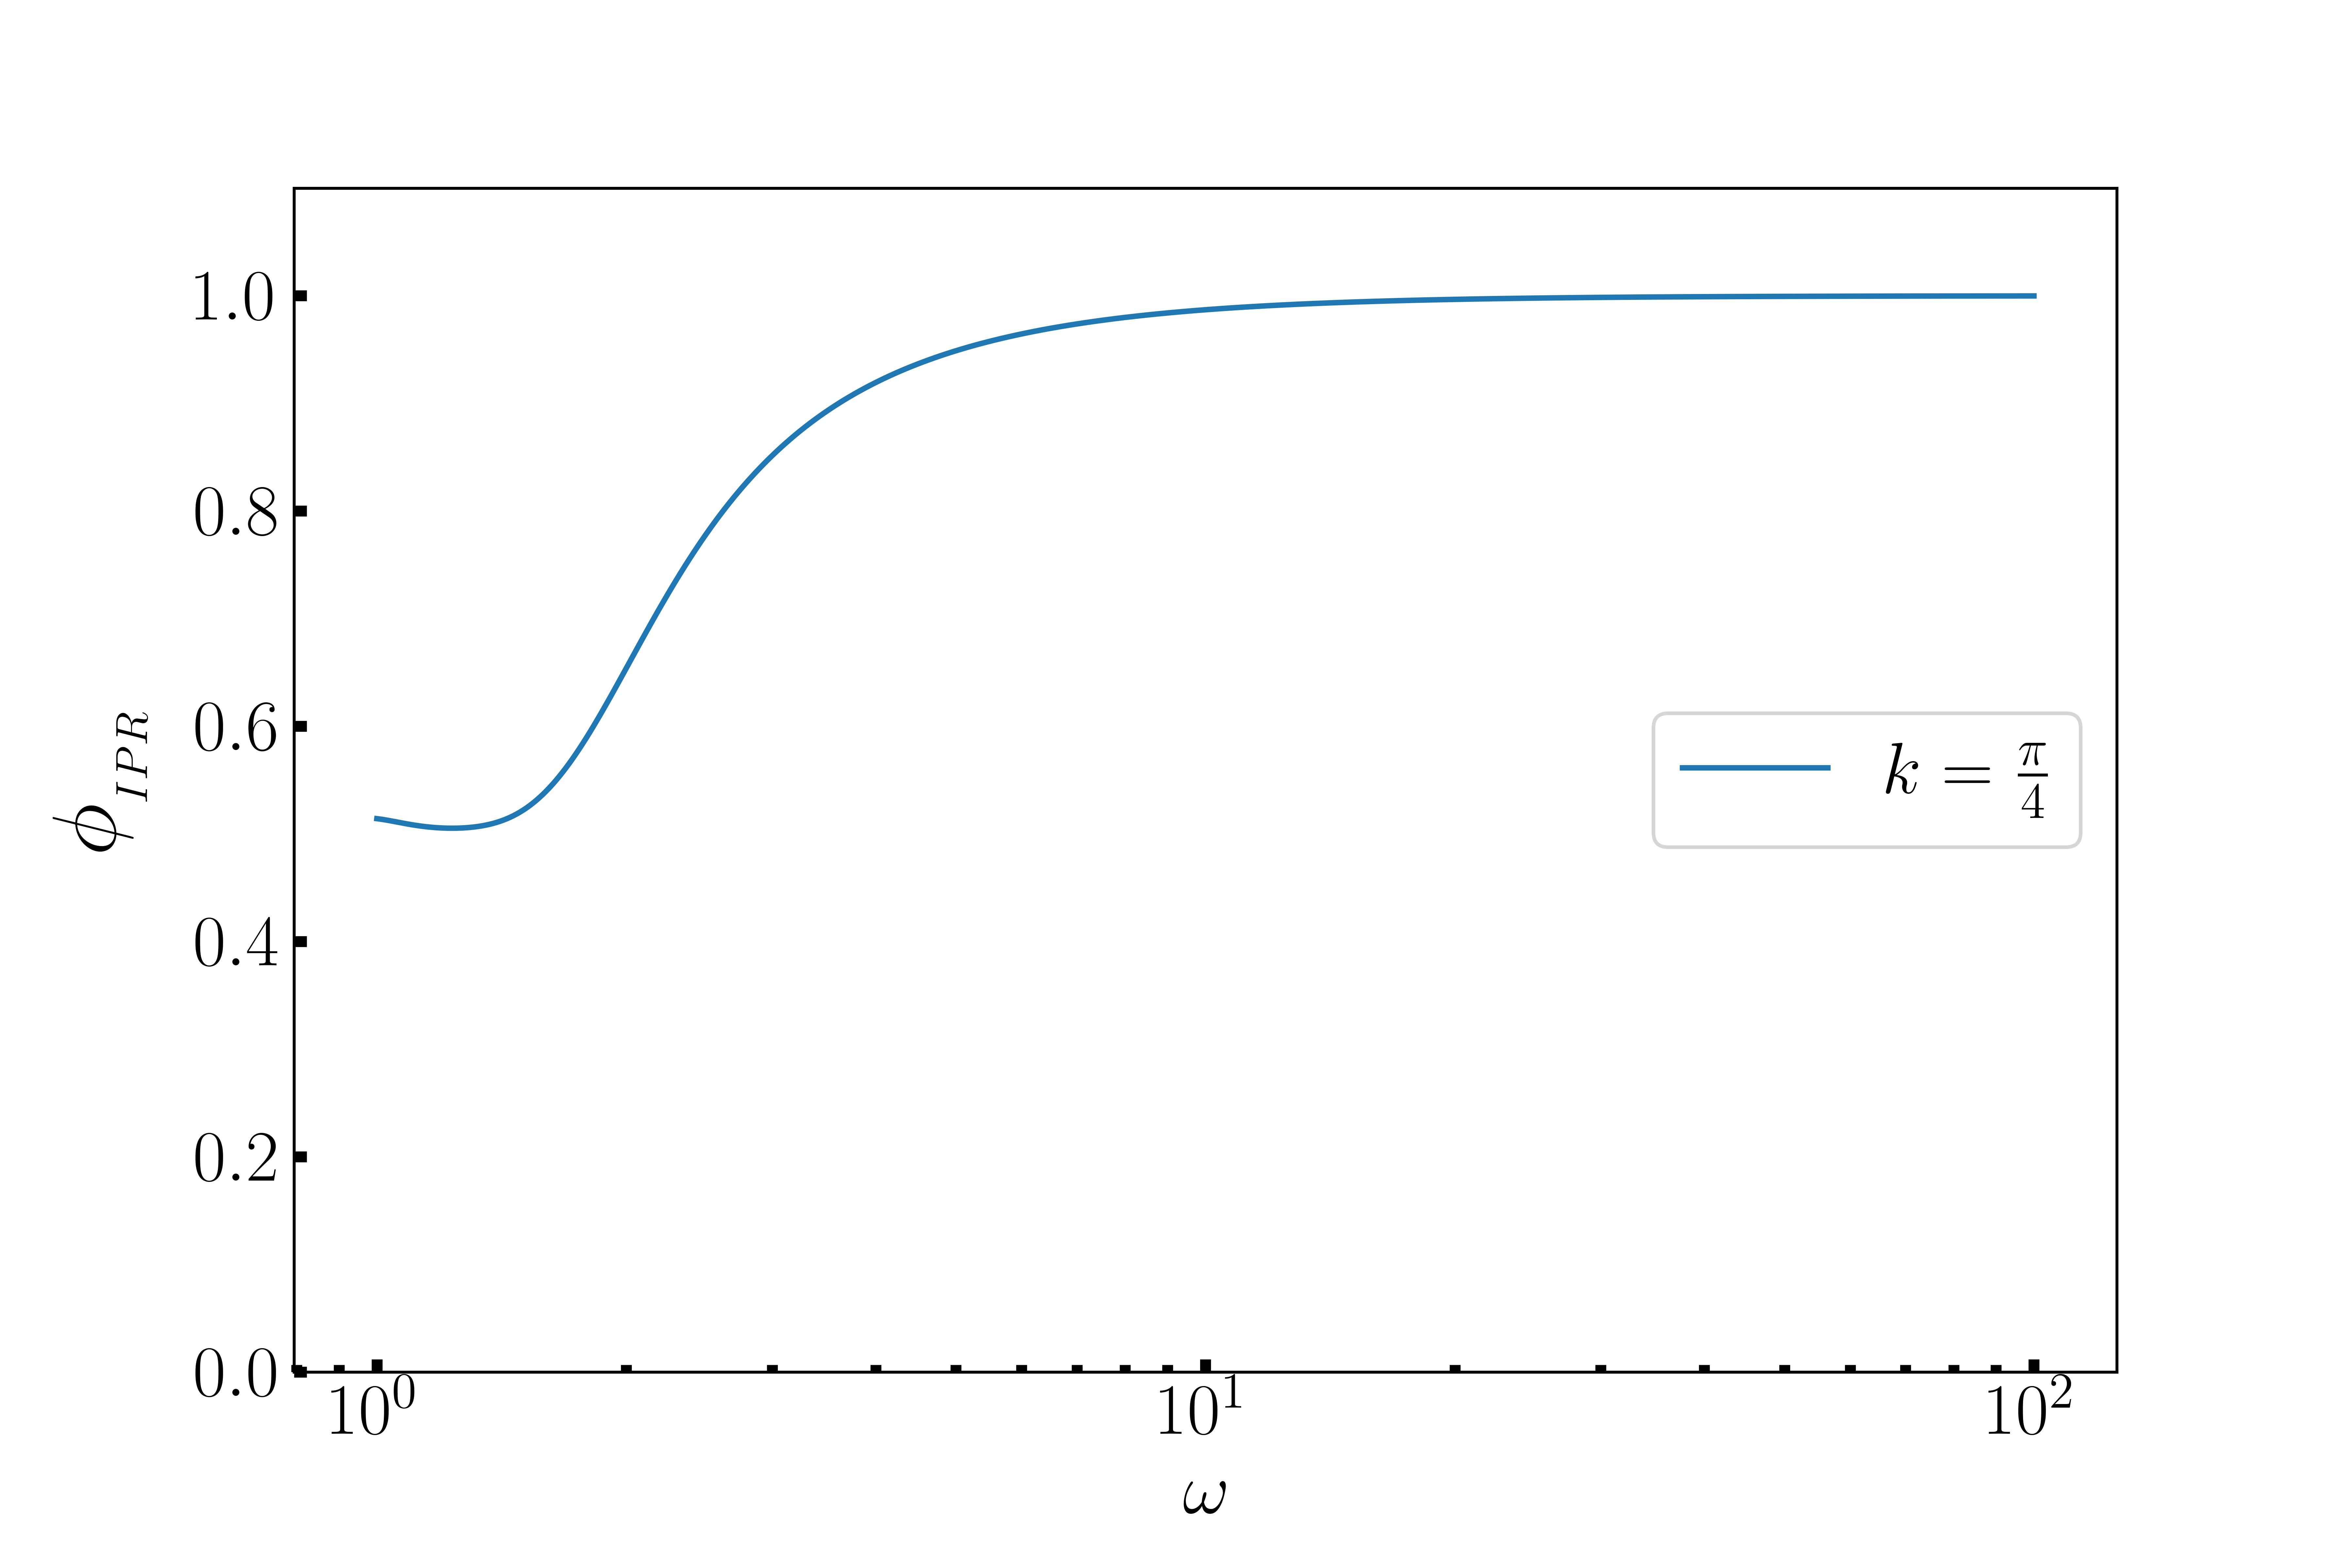
\includegraphics[width = 9.5cm]{phase_transition_ising.jpeg}
		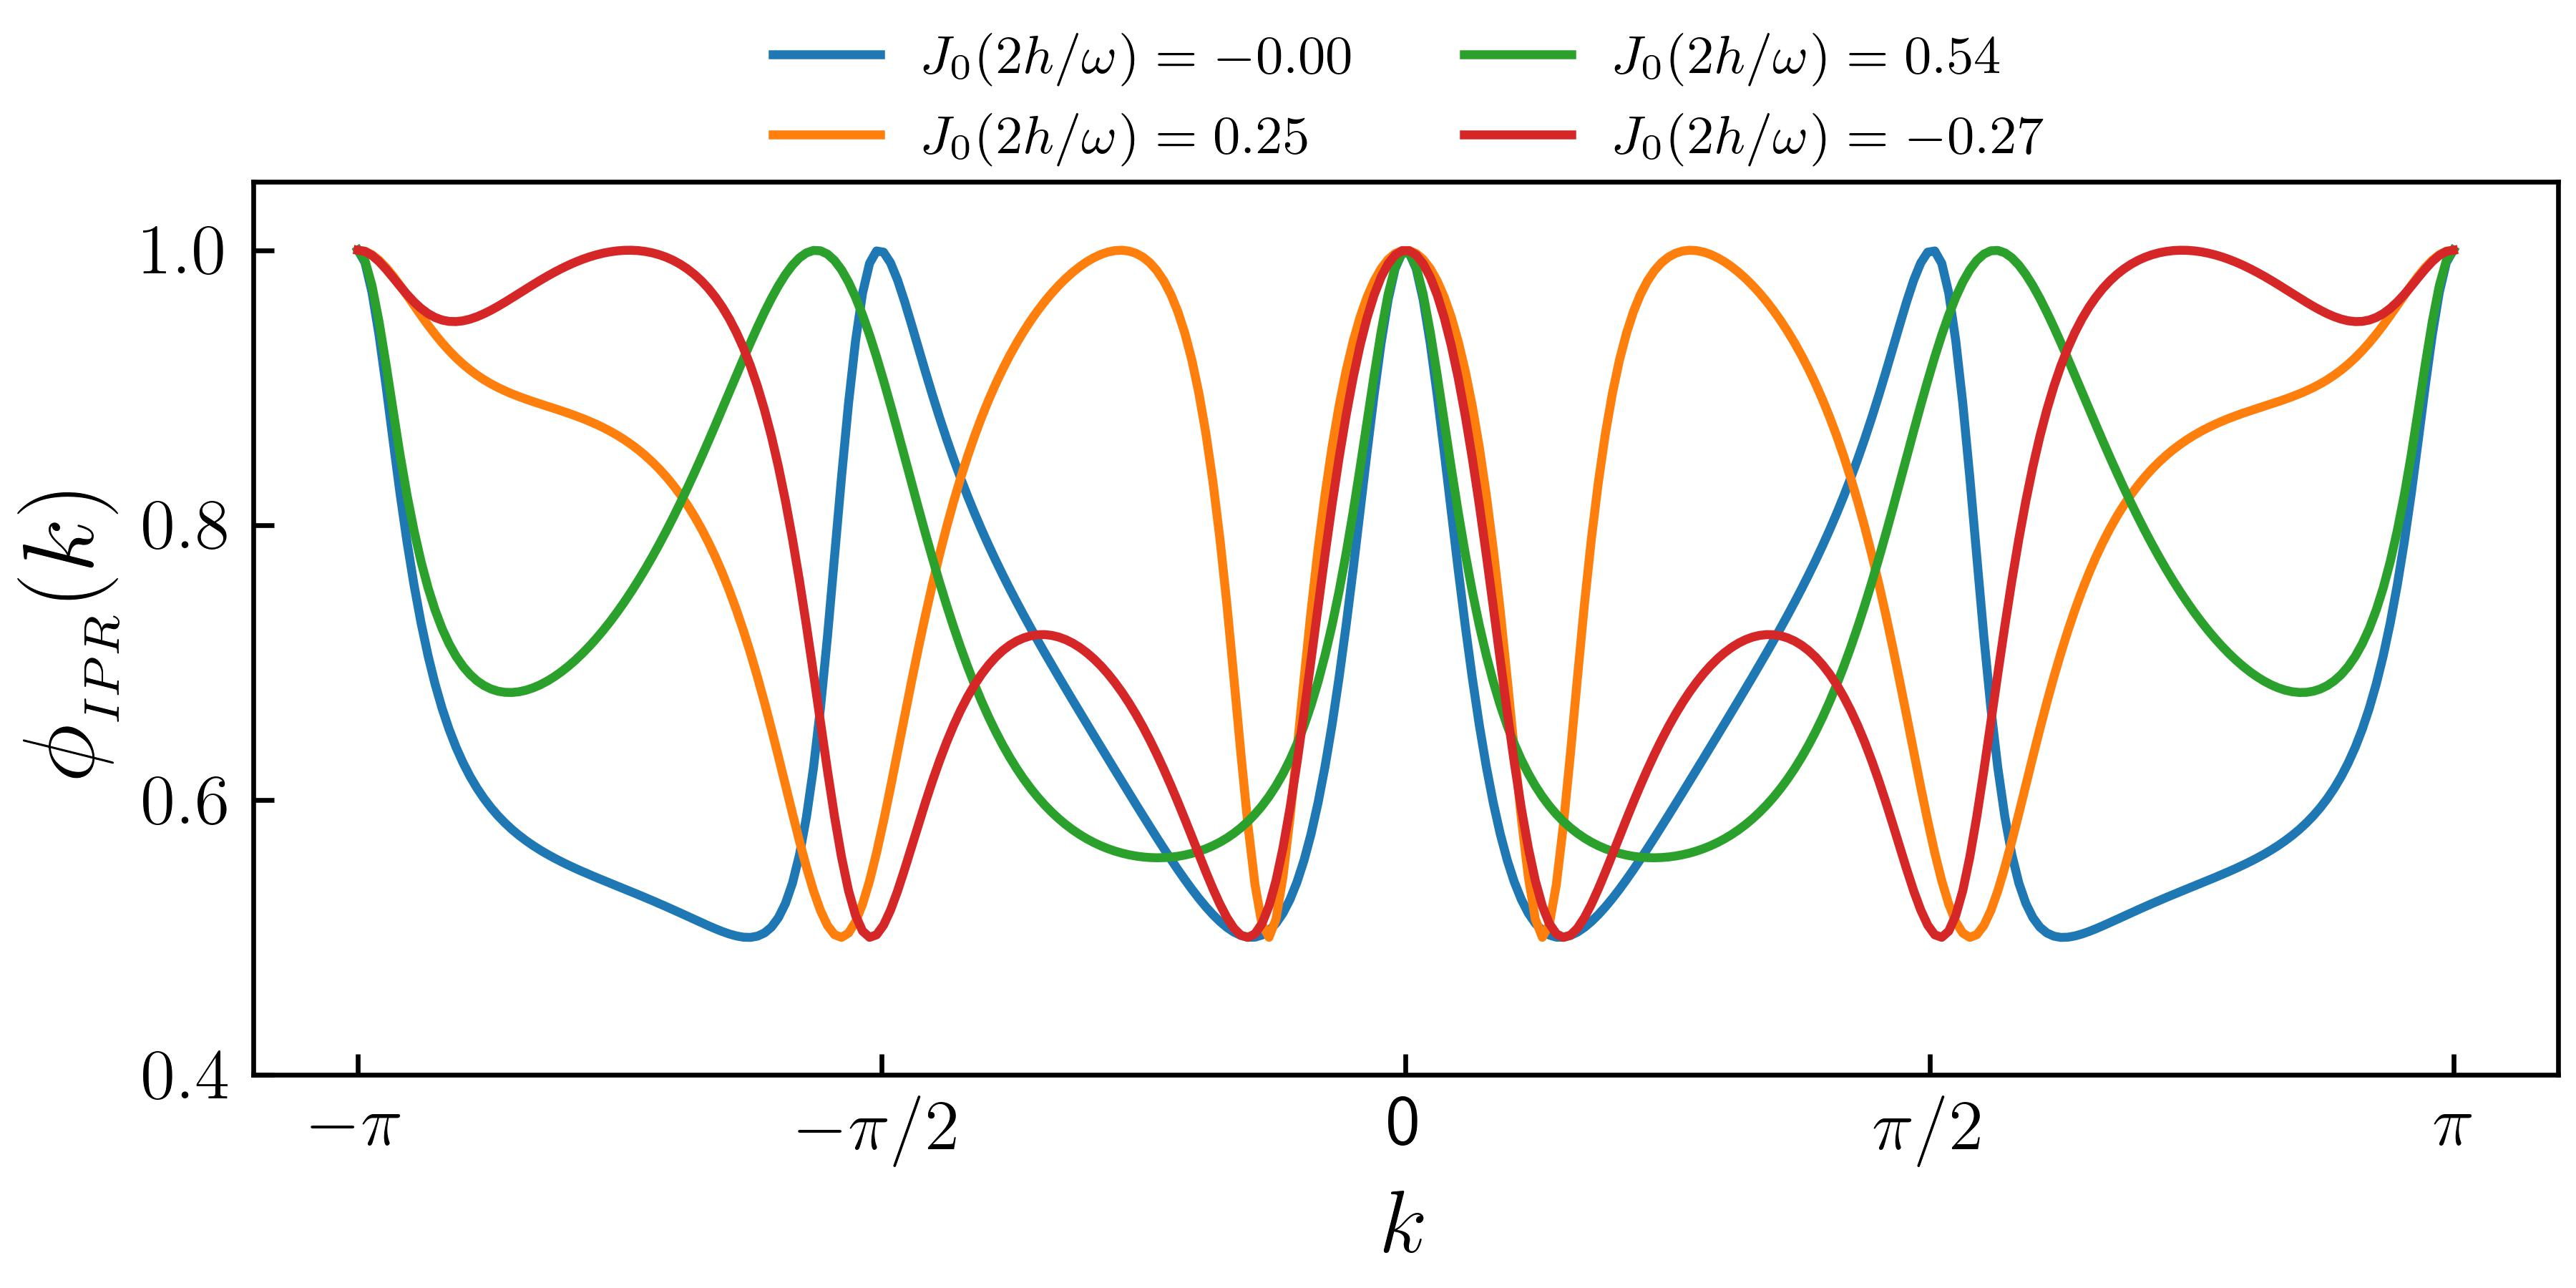
\includegraphics[width = 8.5cm]{ising_exact_lowfr_ipr.jpeg}
		\caption{Reduced IPR obtained by adiabatically increasing $\omega$ (top panel abscissa) for one the floquet mode obtained from equation~\ref{eq:ipr:ising} at the root of $J_0(\eta)$ for N = 500. IPR is $\sim 0.5$ (localized yet no freezing) upto $\omega \sim 2$, afterthat, smoothly increased to unity (fully localized and freezibg) at higher $\omega \geq 10$ (top panel, ordiante). At bottom panel cros-sections for four chosen amplitudes at $\omega =2$ are plotted for a brillouin zone (abscissa) with corresponding reduced IPRs(ordinate).}
		\label{fig:ipr:isinglowfrk}
	\end{figure}
	
	Because the dependence of observable expectations on the eigenstates is always fairly strong for integrable systems like the TFIM, such systems will never exhibit any kind of thermal behaviour unless integrability breaking terms (such as strong disorder) are included~\cite{roy_fate_2015}. As a result, it is not physically meaningful to refer to the unit IPR region as "\emph{Many Body Localization}", because the parameter space lacks a thermalized region to contrast with this state. The type of Floquet Engineering described above, on the other hand, can be easily applied to a broad class of nonintegrable systems where FETH is expected to hold in certain regions. Long-range spin systems, in particular, where the exchange energies between far-off spins are taken into account in the model Hamiltonian, are good candidates because they are known to thermalize when driven with low frequencies~\cite{russomanno_thermalization_2015}.
	\section{\label{sec:level3}Lipkin Meshkov Glick Model: Long range interaction}	
	The periodically driven Curie-Weiss model for $N$ long-range spins is described by the Hamiltonian

	\begin{equation}
		\hat{H}(t) = \hat{H}_0 + \big[h \cos{(\omega t)} + h_0\big]\; \hat{H}_1.
		\label{eq:driven:ham}
	\end{equation}
	Here, the undriven part $\hat{H}_0$ and the driven part $\hat{H}_1$ are, respectively, 
	\begin{eqnarray}
		\label{eq:curieweiss:ham}
		\hat{H}_0 &=& \frac12 \sum_{ij}J_{ij}\hat{\sigma}^z_i\hat{\sigma}^z_j,\\
		\hat{H}_1 &=& \sum^N_{i=1}\hat{\sigma}^x_i.\nonumber
	\end{eqnarray}
	The Heisenberg exchange energy of the bond between spins $i$ and $j$ is given by
	\begin{equation}
		\label{eq:jij}
		J_{ij} =\frac{J_\alpha}{N^{1-\alpha}}\frac{1}{r_{ij}^{\alpha}},
	\end{equation}
	with $r_{ij}$ representing the smallest graph distance between them.
	Putting  $\alpha = 0$ yields the Lipkin Meshkov Glick (LMG) model with all-to-all interaction, yielding $J_{ij} = J_0/N$. We choose to maintain the extensivity of the interaction energy by enforcing the condition
	\begin{equation*}
		\frac{J_0}{N} \sum_{i\neq j}1=\frac{J_0}{N}\frac{N(N-1)}{2}=1,
	\end{equation*}
	yielding the Kac-norm $J_0=2/(N-1)$. The Hamiltonianin equation \ref{eq:driven:ham} commutes with $P_{ij} \equiv \displaystyle\frac{1}{2}\left(1+ \vec{\sigma}_i\cdot\vec{\sigma}_j\right)$. In addition, the conservation of total angular momentum $S^2 = \abs{\vec{S}}^2$, with $\vec{S}=S^x\hat{x}+S^y\hat{y}+S^z\hat{z}\equiv\frac12 \sum_i \vec{\sigma}_i$ is assured by the identity
	$\comm{S^2}{H(t)}=0$. We now choose to populate the system in a state with $S^2=\displaystyle\frac{N}{2}\left(\frac{N}{2}+1\right)$. In that case, the dynamics remains invariant in the  $N+1-$dimensional space spanned by the common eigen states of $P_{ij}, \abs{S}^2$ and $S_z$; these are also eigenstates in the so-called TSS subspace ~\cite{mori_prethermalization_2019}. Let the eigenvalues be $s_n$, and the eigen vectors be $\ket{s_n}$, where $s_n=-\frac{1}{2}+\frac{n}{N}$ and the index
	$n= 0 (1) N$ has $N+1$ values. The dynamics is restricted to this invariant subspace, wherein the matrix elements of the Hamiltonian are given by
	
	\begin{align}
		(H_0)_{ij} &= -\frac{4}{N-1} s^2_i \delta_{ij},\nonumber\\
		(H_1)_{ij} &= \Bigg[\sqrt{\frac{N}{2}\left(\frac{N}{2}+1\right) - Ns_i(Ns_{i + 1})}\delta_{i+1, j} \nonumber\\ 
		&\hskip 0.7cm +\sqrt{\frac{N}{2}(\frac{N}{2}+1) - Ns_i(Ns_{i- 1})}\delta_{i-1,j}\Bigg]
		\label{eq:lmg:tssham}
	\end{align}
	Now we transform the Hamiltonian to the Rotated frame given by the transformation
	
	\begin{equation}
	\hat{U}(t)=\exp [i \frac{h}{\omega} \sin (\omega t) \hat{H}_{1}]
	\end{equation}
	Defining $\tau = \displaystyle\frac{h}{\omega}\sin{\omega t}$, we use the fact that $\hat{H}_1 = 2 S^x$, and the following identity obtained using the Baker-Campbell-Hausdorff formula,
	\begin{equation}
	e^{i 2\tau\hat{S^{x}}} \hat{S^{z}} e^{-i 2\tau \hat{S^{x}}}=\hat{S^{z}} \cos \left(2\tau\right)+\hat{S}^{y} \sin (2\tau),
	\end{equation}
	to simplify the transformed Hamiltonian $\tilde{H} = \hat{U}\hat{H}\hat{U}^\dagger - \hat{U}^\dagger\partial_t\hat{U}$, yielding
	
	\begin{align}
		\tilde{H}(t)& = -\frac{1}{N-1}\Big[\big(S^z\big)^2 \big(1+\cos{4\tau}\big)+ \big(S^y\big)^2 \big(1-\cos{4\tau}\big)\nonumber \\  
		&\hskip 2.5cm + \pb{S^y}{S^z}
		\sin{4\tau}\Big] - 2 h_0 S^x
	\end{align}
	
	
	We define $\eta\equiv 4h/\omega$ and use the Jacobi-Anger formula in eqn~\ref{eq:jacobi}
	to simplify the expression for $\tilde{H}(t)$, then 
	assume that $\omega$ is large enough to smooth out the harmonic components present in the Hamiltonian. Ignoring constant terms, this yields
	\begin{equation}
	\tilde{H}_{\mathrm{RWA}}= \frac{\big(\hat{S}^x\big)^{2}}{N-1} - 2h_0 \hat{S}^x - \frac{J_0(\eta)}{N-1}\bigg[\big(\hat{S}^z\big)^{2} - \big(\hat{S}^y\big)^{2} \bigg]
	\end{equation}
	\todo{Proofread from here}
	
	If the drive amplitude $h$ is adjusted such that $\eta$ lies at a root of $J_0(\eta)$ (the localization point), the RWA Hamiltonian is diagonal in the representation of the transverse field $\hat{S}^x$, yielding an IPR of unity in that representation, similar to the Ising case. Note however, that if the DC transverse field $h_0$ is set to $0$, then, at the localization point, the RWA Hamiltonian $\tilde{H}_{\mathrm{RWA}}\sim
	\big(\hat{S}^x\big)^2$, each of whose eigenvalues (given by $\big(\frac{N}{2}-m\big)^2$ where $m \in 0(1)N$, and $\big(\frac{N}{2}-m\big)$  are the eigenvalues of $\hat{S}^x$) are two-fold degenerate. This produces infinitely many (Floquet) eigenmodes in the degenerate subspace whose IPRs may not always be unity in the $S^x$ representation. Thus, the absence of the DC field may produce delocalization in the Floquet states even at the localization points, and this necessitated the inclusion of a DC field $h_0$ in order to break the symmetry.
	Finally, note that not all values of the DC field $h_0$ remove all degeneracies in $\tilde{H}_{\mathrm{RWA}}$. To see this, note that, at the localization point, the eigenvalues of $\tilde{H}_{\mathrm{RWA}}$ are given by
	
	\begin{equation}
	\rm{Eigs}\bigg[\tilde{H}_{\mathrm{RWA}}\bigg] = \frac{\big(\frac{N}{2}-m\big)^2}{N-1} - 2h_0 \bigg(\frac{N}{2}-m\bigg)
	\end{equation}
	
	In order to ensure that no degeneracies occur, we have to adjust $h_0$ to ensure that for any two integers $m_1, m_2 \leq N$  the condition following is always met,
	
	\begin{equation}
	\frac{\big(\frac{N}{2}-m_1\big)^2}{N-1} - 2h_0 \bigg(\frac{N}{2}-m_1\bigg) \neq \frac{\big(\frac{N}{2}-m_2\big)^2}{N-1} - 2h_0 \bigg(\frac{N}{2}-m_2\bigg)
	\end{equation}
	
	If $N\gg 1$ (substantially large), then this condition can be met by assuring that $(1-2h_0)^{-1}$ is never an integer that is divisible by $N$. To ensure this in our numerical simulations we have kept $h_0$ at a small irrational value.
	
	
	This result is supported by exact numerical results, as can be seen in the plots below in FIG. \ref{lmg_ipr_exact}. There, we show plots of the IPR of the Floquet mode $\ket{\phi^n}$ for all $n$ corresponding to eigenvalues of $S^x$ for a fixed eigenvalue of $S^2 = N/2\big(N/2 + 1\big)$. The IPR is thus
	\begin{equation}
	\phi_{IPR}(n) = \sum_m \abs{\ip{m}{\phi^n}}^4
	\label{iprlmg}
	\end{equation}
	where $|m\rangle$ is the $m^{th}$ eigenstate of $\hat{S}^x$.
	
	
	Now, we focus at numerical simulations for $H(t)$ via the IPR of the Floquet state in the representation of the transverse field i.e. the eigenstates of $S^x$. We kept frequency $\omega = 90$ as a large enough value for RWA to hold, and $N=\mathcal{O}(10^2)$ which our standard computational resources will allow. 
	
	\begin{figure}[]
		\centering
		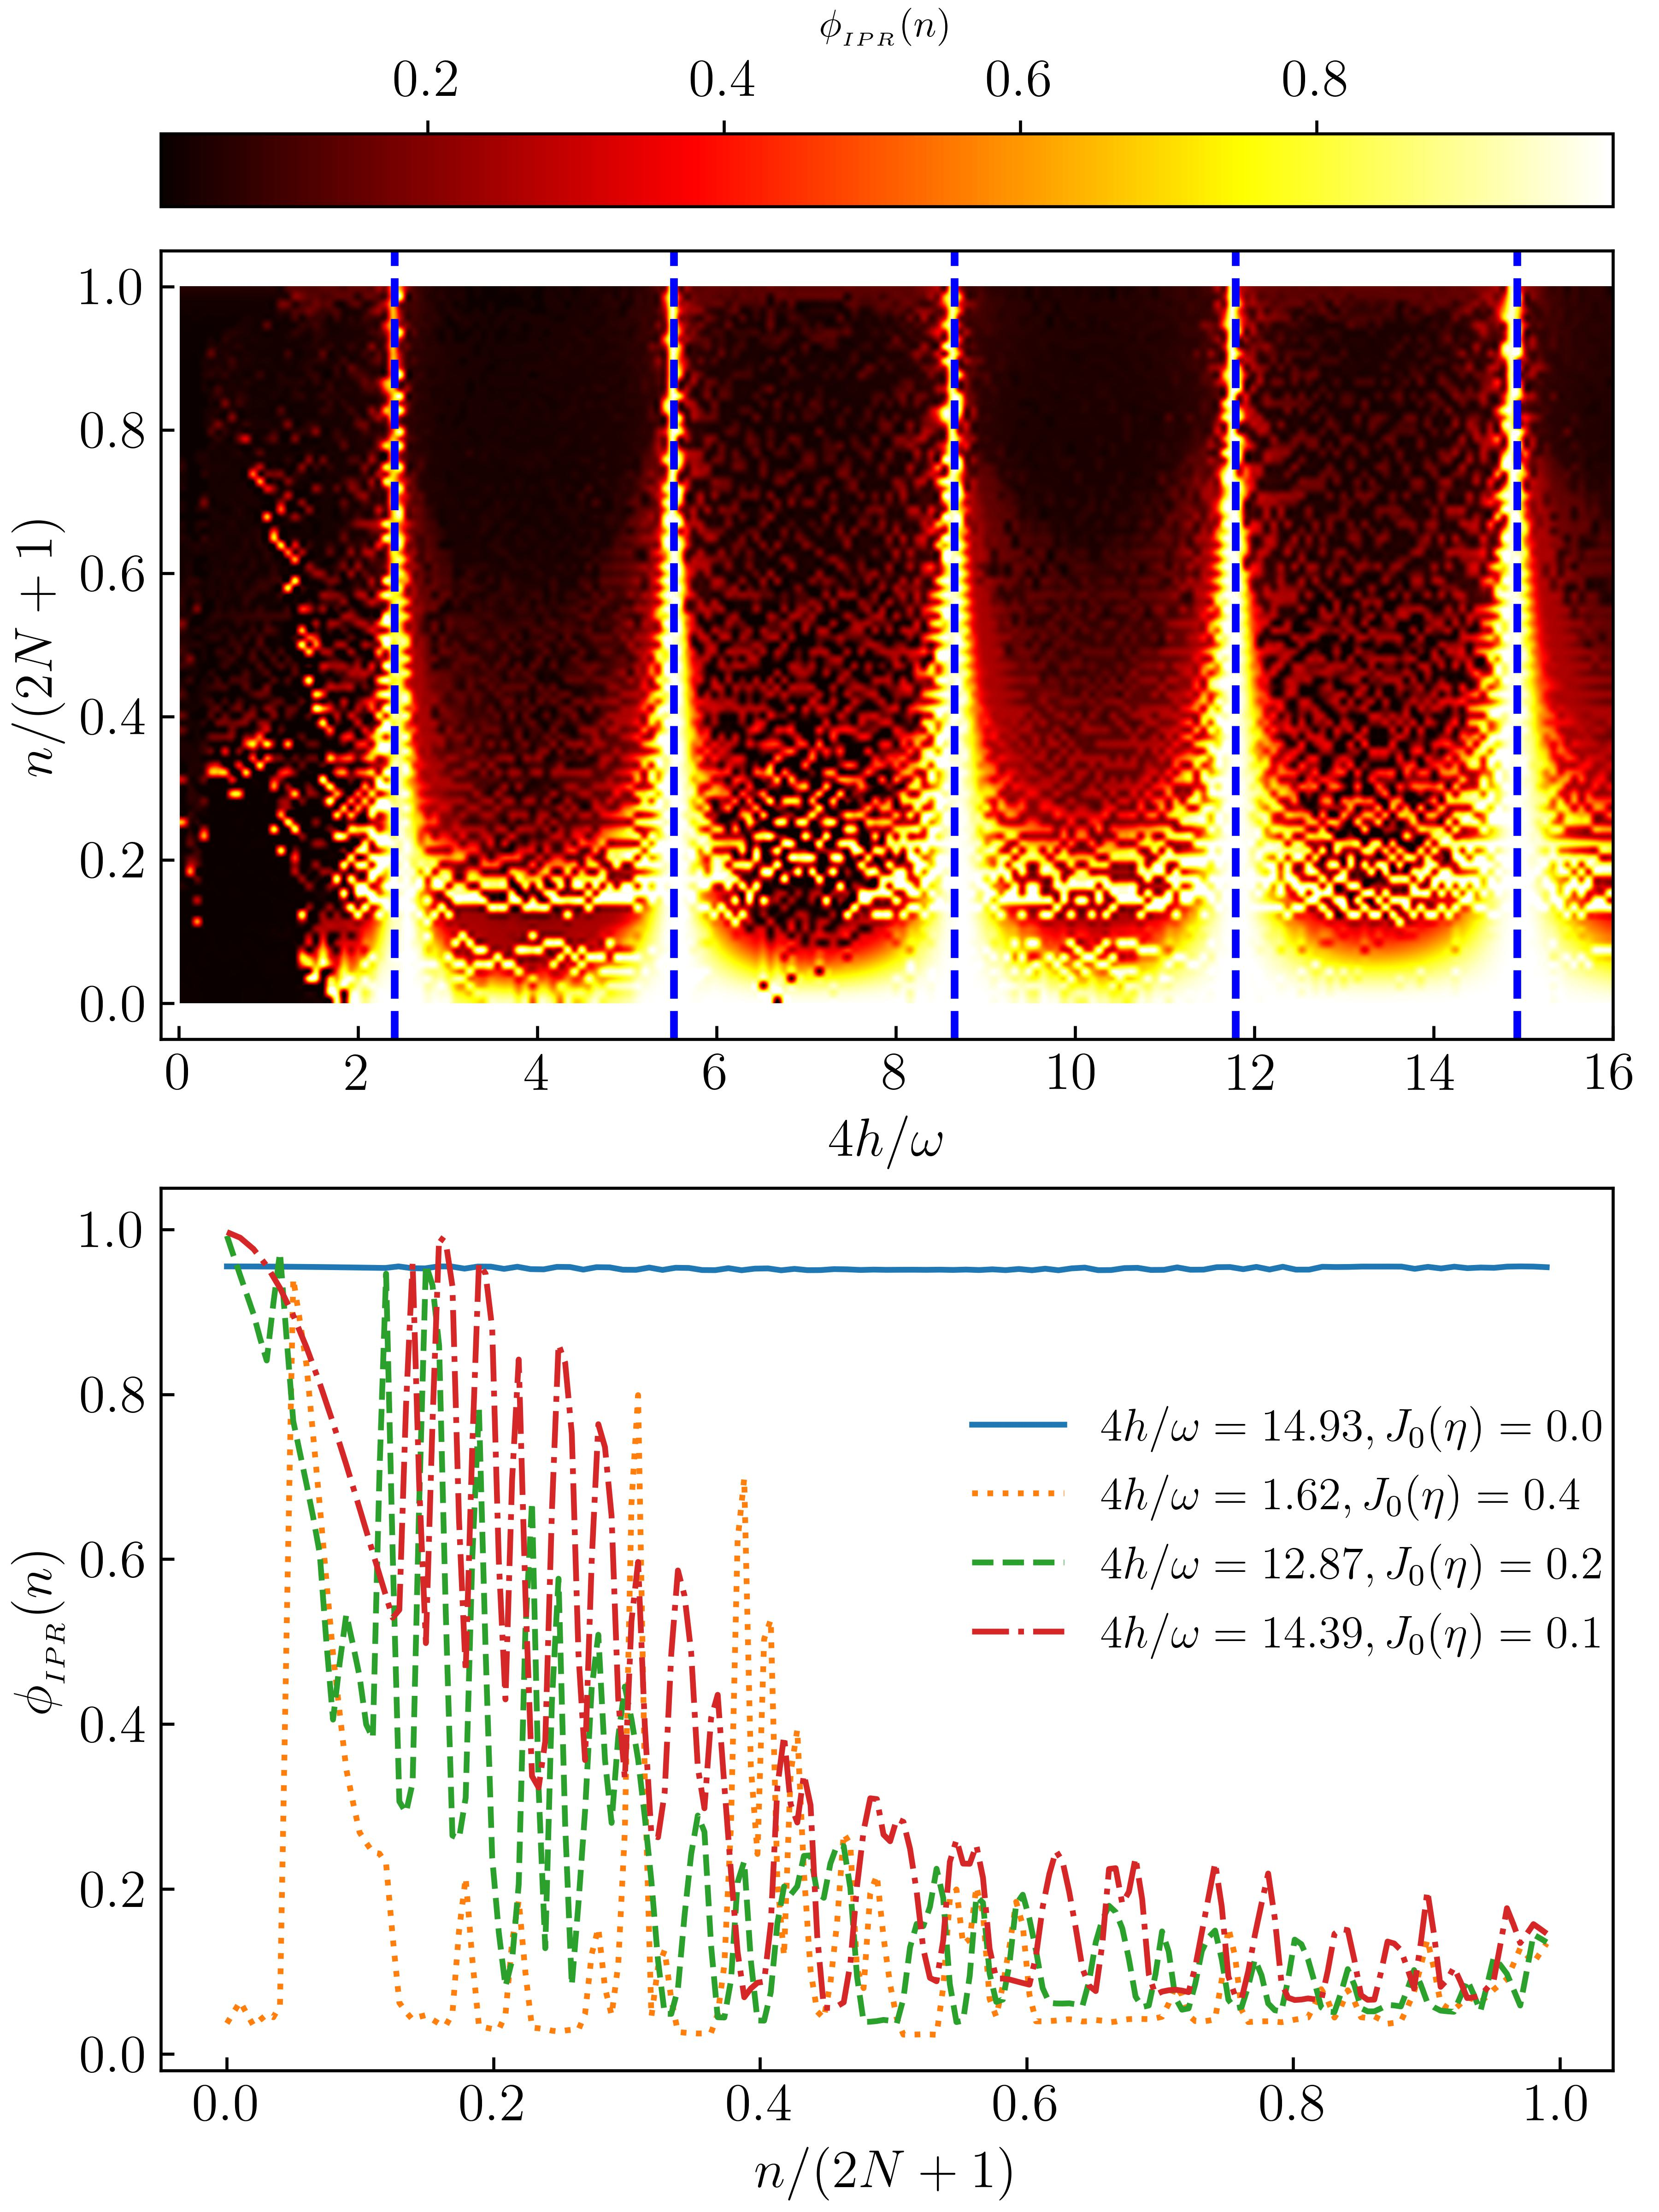
\includegraphics[width = 8.5cm]{ipr_exact_dynm_N50_frq_90_.jpeg}
		\caption{IPR density plot for all possible flquet modes (top panel ordinate) for different values of $\eta = 4h/\omega$ (top panel abscissa), deduced from equation \ref{iprlmg} for exact LMG Hamiltonian for N = 50. Blue dashed lines are roots of $J_0(\eta)$. At bottom panel cross-section of IPR (ordinate )for four different $\eta$'s plotted for all possible floquet modes(bottom panel, abscissa) at $\omega=90$. IPR founds to be $\sim$ unity for all floquet modes at roots of $J_0$.}
		\label{lmg_ipr_exact}
	\end{figure}

	The uppermost section displays a density plot that depicts the Inverse Participation Ratio (IPR) of the Floquet states in FIG\ref{lmg_ipr_exact}. The abscissa represents $\eta=4h/\omega$, while the ordinate represents the spin index \emph{m/(2N+1)}. The vertical lines that are dashed and colored blue correspond to the roots of the Bessel function of the first kind with order zero, denoted as $J_0(\eta)$. Evidently, the Inverse Participation Ratio (IPR) approaches a value of one for high values of the root of the Bessel function $J_0(\eta)$, which suggests a state of full localization of the Many Body system. Nevertheless, a deviation from unity occurs at the smallest root of $J_0(\eta)$. The observed phenomenon can be attributed to the fact that when $\eta$ approaches the smallest root of $J_0(\eta)$, which is approximately equal to $2.405$, the amplitudes of the higher order terms in the RW expansion, denoted by $\mathcal{O}(J_n(\eta))$, become significant enough to contribute to the process of delocalization.  Thus, a greater magnitude of the root is favored for the purpose of investigating the phenomena.
	
	The bottom panel contains cross sections of the full IPR plot for selected values of $\eta$ as indicated in the legend. When the drive amplitude $h$ is adjusted to make $J_0(\eta)\neq 0$, the Floquet States are mixed, but not entirely thermal, since the IPR does not fall to $\mathcal{O}(N^{-1})$, indicating that localization persists to some extent always. So, as long as there is an appropriate DC field, $\hat{S^x}$ is mostly conserved and $\hat{H}_F$ is mostly diagonal in the $\hat{S^x}$ representation at the freezing point. The small deviations from this conservation occur due to the role of higher order terms in the Fourier expansion of the Hamiltonian on the rotating basis that contribute additional time-periodic terms to the RWA Hamiltonian, as can be seen in FIG.\ref{lmg_ipr_rwa11}.
	
	The full Hamiltonian for the LMG model on the rotated basis is
	\begin{widetext}
		\begin{multline}
			\tilde{H}^{RWA}(t)\sim \frac{\big(\hat{S}^x\big)^{2}}{N-1} - 2h_0 \hat{S}^x - \frac{J_0(\eta)}{N-1}\bigg[\big(\hat{S}^z\big)^{2} - \big(\hat{S}^y\big)^{2} \bigg] - \frac{2}{N-1}\sum^\infty_{n=1}\;J_{2n}(\eta)\;\Big[\big( \hat{S}^z\big)^2 - \big( \hat{S}^y\big)^2\Big]\;\cos{\big(2n\omega t\big)}\\
			- \frac{2}{N-1}\sum^\infty_{n=1}J_{2n-1}(\eta)\;\big\{ \hat{S}^y,  \hat{S}^z \big\}  \;\sin{\Big[\big(2n-1\big)\omega t\Big]}
		\end{multline}
	\end{widetext}
	
	\begin{figure}[ht!]
		\centering
		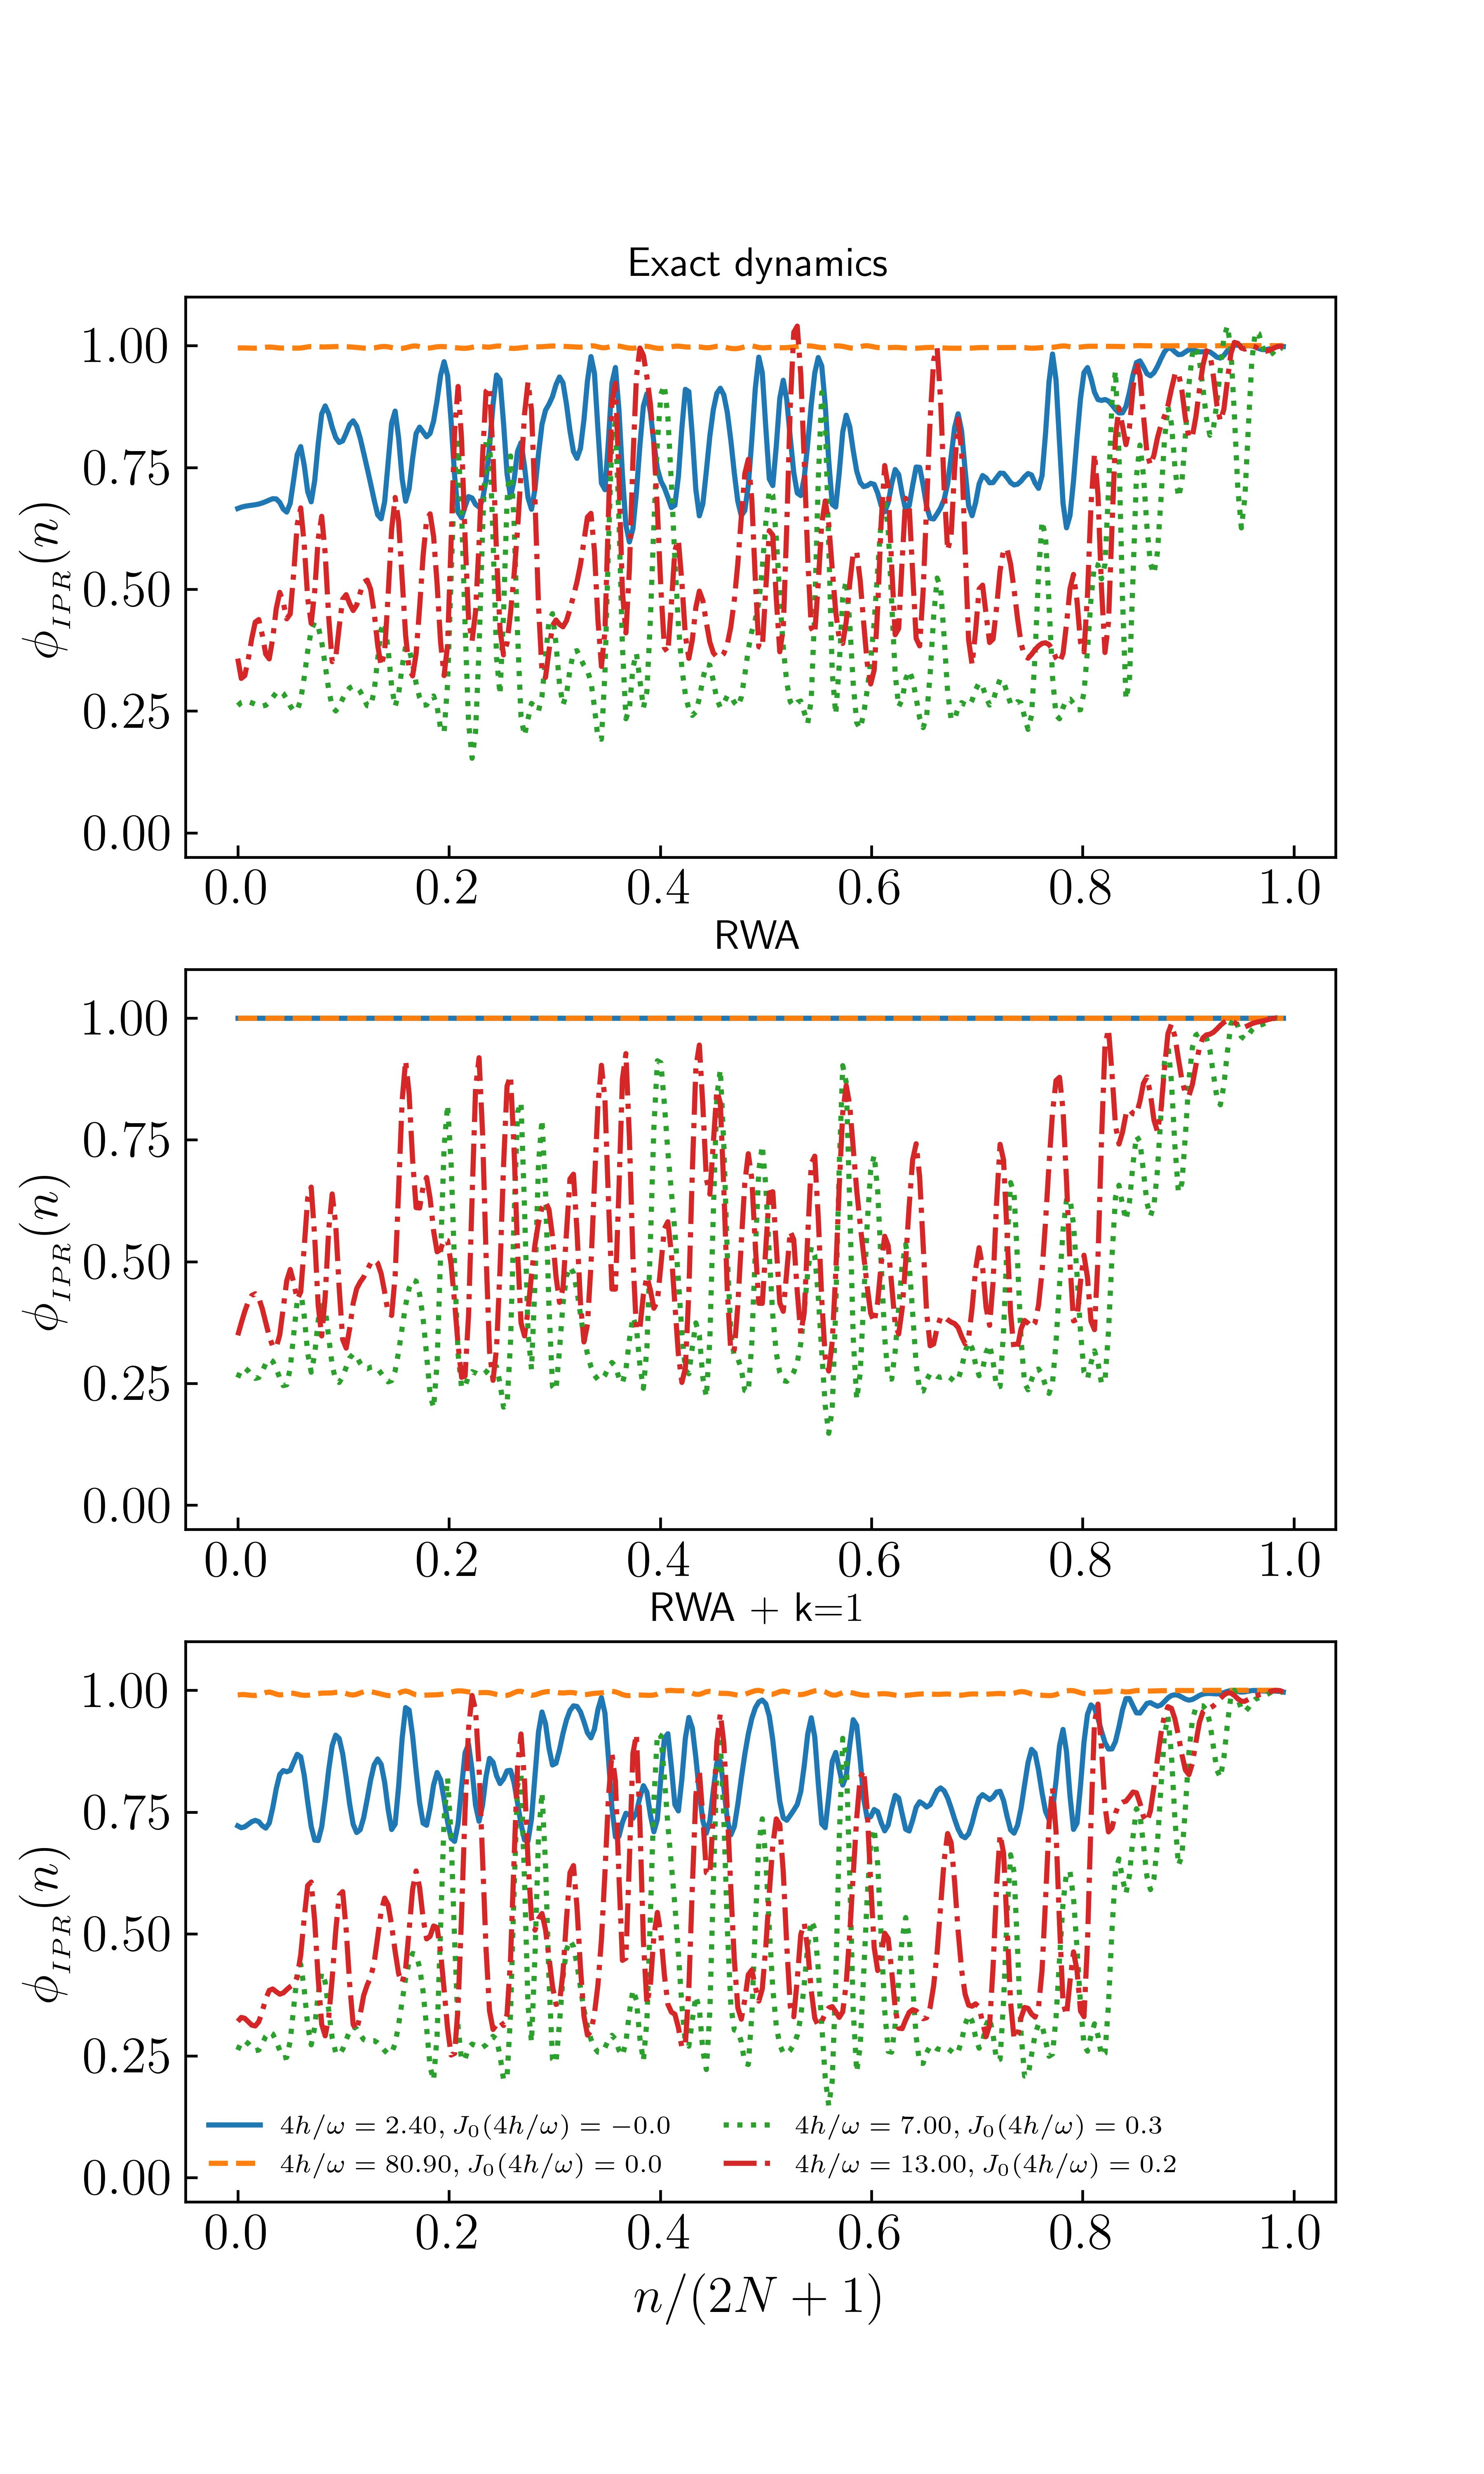
\includegraphics[width =9.0cm]{comprasion_LMG_50_highFr90_exact_nd_rwa.jpeg}
		\label{lmg_ipr_rwa11}
		\caption{The comparison between IPR for exact dynamics and RWA with corresponding correction orders. IPR is calculated for four different $\eta$'s and corresponding $J_0(\eta)\neq 0$ values for colors, Blue :$\eta = 2.40, J_0(\eta) = 0.0$, dashed orange:$\eta = 18.07, J_0(\eta) = 0.0$, Green:$\eta =13.03, J_0(\eta) = 0.21$, Red:$\eta = 1.62, J_0(\eta)= 0.44$. IPR plots for RWA with zeroth order aren't enough to describe the exact dynamics, but plots for RWA with first-order correction are similar to the exact dynamics.}
	\end{figure}
	
	The IPR plots pertaining to exact dynamics indicate that the freezing point, represented by the initial blue curve corresponding to Bessel's root of zeroth order of first kind, is insufficient for achieving many-body localization, as depicted in the top panel. The reason for this phenomenon is attributed to the greater magnitude of other Bessel roots of higher order, which in turn leads to delocalization. However, it is worth noting that at elevated localization points (as depicted by the dashed orange curve), localization is particularly conspicuous. In terms of system distribution, a range of curves, denoted by both green and red, illustrates the degree of distribution. The zeroth order RWA in the central panel exhibits a consistent pattern at locations distant from the resonance point, as evidenced by the congruent green and red curves. However, the curves for both higher and lower localization points display complete localization, which contradicts the precise findings presented in the top panel. This necessitates the incorporation of higher-order corrections into the Rotating Wave Approximation (RWA). The application of the first-order correction to RWA in the lower panel results in a curve structure that is recognizable and consistent with the exact dynamics.
	
	\section{\label{sec:level4}Classical Lipkin Dynamics}
	In the context of the classical (continuum) limit, where $N$ approaches infinity, the disparity between neighboring values of $s_i$ in equation \ref{eq:lmg:tssham} can be disregarded, resulting in a Hamiltonian per particle of $h(t)\equiv \frac{1}{N}$ and the Hamiltonian per particle becomes
	
	\begin{equation}
	h(t)\equiv \frac{1}{N}H(t) = h + h_0\cos{(\omega t)}h_1,
	\end{equation}
	where,
	\begin{eqnarray}
	(h)_{ij} &\approx& - 2s^2_i \delta_{ij},\nonumber\\
	H_0 &\rightarrow& -2s^2\nonumber\\
	(h_1)_{ij} &\approx& \sqrt{1 - 4s^2_i}\left[\delta_{i+1, j}  + \delta_{i-1,j}\right]\nonumber\\
	H_1 &\rightarrow& \sqrt{1 - 4s^2_i}\cos{p},
	\end{eqnarray}
	
	In the continuum limit, the Lipkin system can be described by $p,q$ with corresponding Hamiltonian ~\cite{sciolla_quantum_2010}:
	\begin{equation}
	H = -2 q^2 - h(t)\;\sqrt{1-4q^2}\;\cos{p},
	\label{eq:class:ham}
	\end{equation}
	which yields the Hamiltonian dynamical system 
	\begin{align}
		\dv{q}{t} &= h(t)\sqrt{1-4q^2}\sin{p}\nonumber \\
		\dv{p}{t} &= 4q\bigg[1-\frac{h(t)\cos{p}}{\sqrt{1-4q^2}}\bigg]
		\label{eq:class:poinc}
	\end{align}
	
	We recovered Hamiltonian numerically \ref{eq:class:ham} using equations \ref{eq:class:poinc} to obtain position and moemntum coordinates $p,q$ and plotted in the \emph{Poincar$\acute{e}$ surface of section} (PSOS) strobbed at integer multiple of time period. A chaotic Poincare pattern is found for all small drive amplitude $s.t.$  $A/J < 0.5 $ and also a regular pattern emerges at for ratios $A/J$ $\geq$ 0.5 both at small drive frequency $\omega \sim 2.0$ ~\cite{russomanno_thermalization_2015}. 
	
	However, under a regime of sufficiently high frequency, the system exhibits distinct behavior. The study involves a comparison of the Poincar$\acute{e}$ sections of the ensuing dynamics under the influence of $h(t)=h\cos{\omega t}$, where two distinct scenarios have been considered. The first scenario pertains to the case where frequency $\omega=2.5$, corresponds to a lower frequency and, consequently, a smaller amplitude. The second scenario pertains to the case where frequency $\omega=90.0$,  corresponds to a higher frequency and, correspondingly, a higher amplitude. Both scenarios have been evaluated at $J_0(4h/\omega)=0$. The Husimi Q-functions of the acquired Floquet States are compared with these. The quantum phase space is characterized by the Spectral Average of the Husimi functions of all the Floquet modes $\ket{\phi^n}$ for a given value of $S^2$. Specifically, for a coherent state $\ket{q,p}$, the corresponding plot is presented in FIG.\ref{fig:classical_lipkin}.
	\begin{equation*}
		H(q,p)\equiv \frac{1}{\big(2N+1\big)\pi}\sum_n \ip{q,p}{\phi^n}\ip{\phi^n}{q,p}
	\end{equation*}
	
	The classical plots are dominated by chaos at low values of $\omega$, as noted in Kidd's work~\cite{Kidd2019}. Conversely, at high values of $\omega$, the Poincar$\acute{e}$ plot exhibits a distinct regular pattern, indicating localization.
	\begin{figure}[ht!]
		\centering
		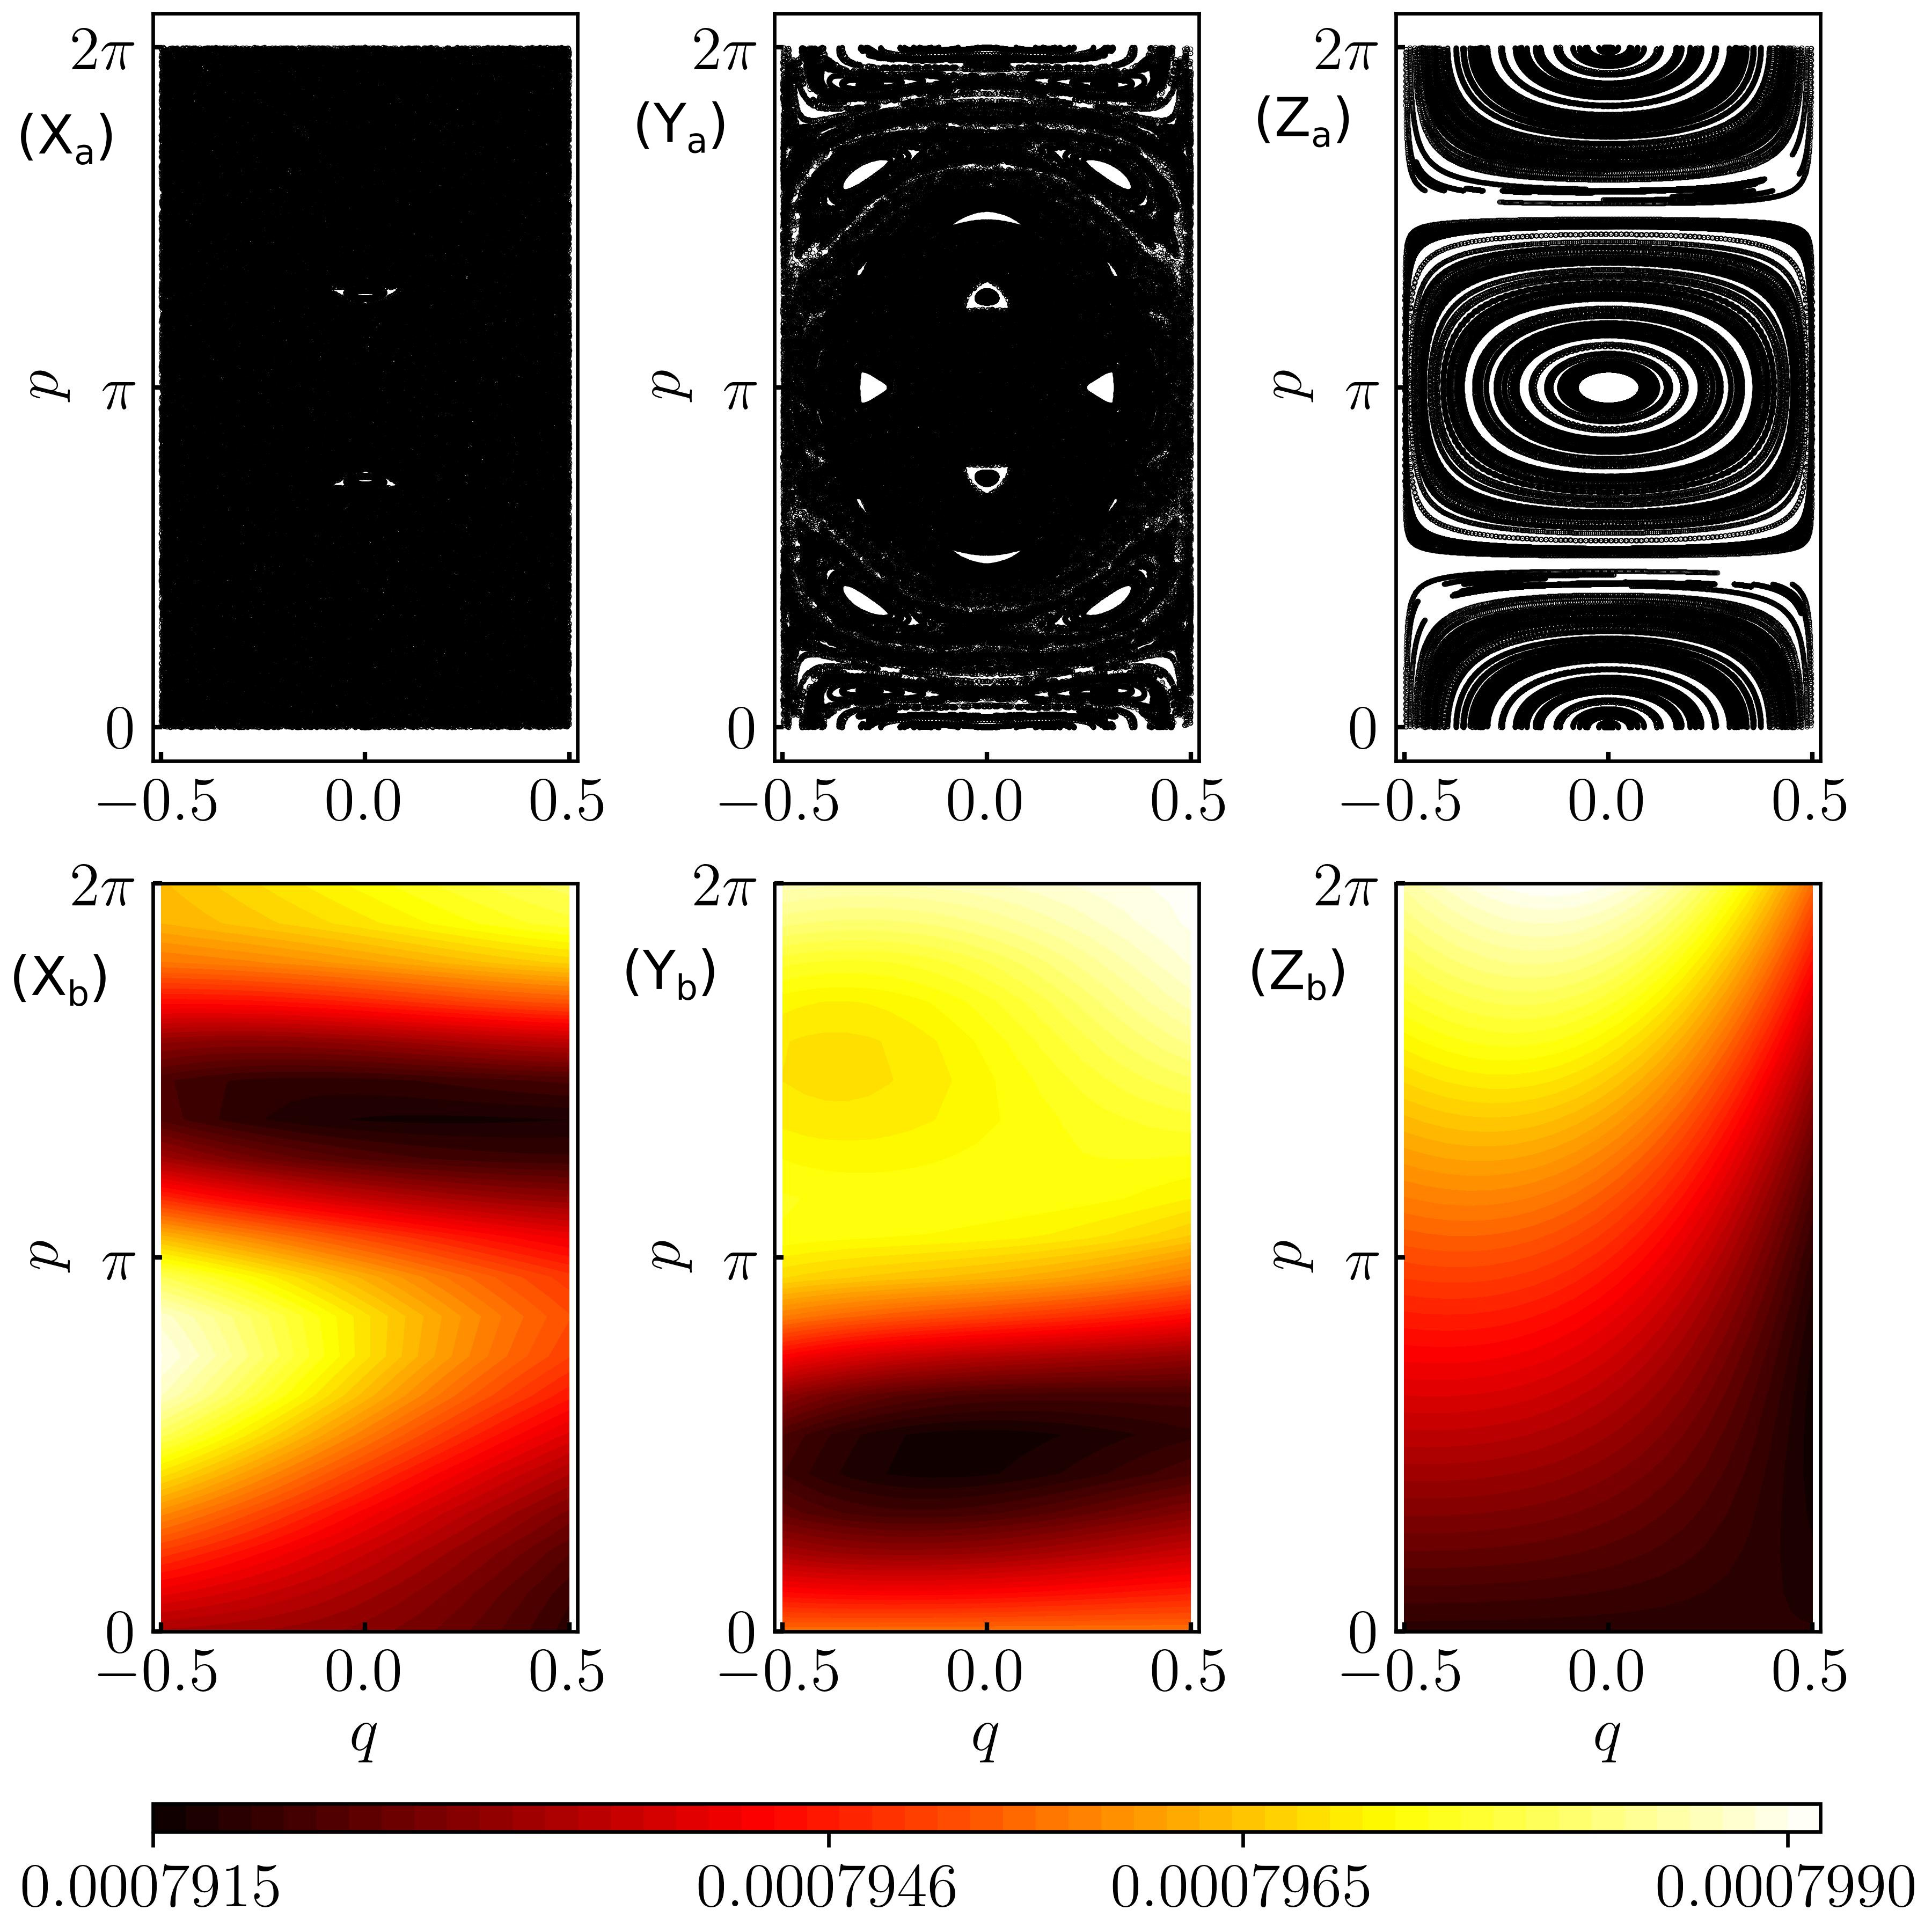
\includegraphics[height = 9.0cm, width = 9.0 cm]{lmg_poincare.jpeg}
		\caption{The above panel describes the phase-space Poincare distribution symmetry breaking smaller drive frequency $\omega = 2.5$ (left) and higher frequency $\omega = 90.0$ (right) for system size $N=500$ with 100 realisation numbers. At smaller frequencies, the Poincare picture contains chaotic behaviour (top left panel) whereas at the higher frequencies, it is a normal Poincare picture which represents discrete freezing behaviour(top right panel). The bottom panel is Hushimi Q-function average plot for  a smaller frequency (bottom left) and has a uniform distribution with less contrast in colour. This means a Q-function distribution in chaotic behaviour. At the right bottom, the Hushimi plot has distinct colour contrast in the Q-function average value which represents a regular dynamics pattern in the system.}
		\label{fig:classical_lipkin}
	\end{figure}
	\section{\label{sec:level5}Thermality to Athermality: A Phase Crossover}
	The analysis of the Lipkin-Glick-Meshkov model reveals two distinct scenarios at low and high external drive frequencies. As a result, it is hypothesized that a change in phase may occur due to the influence of frequency. IPR of the Floquet modes is computed numerically and plotted in FIG.\ref{fig:phase_transition} for numerous frequencies in ascending order from frequency $\omega = 1.0$ upto $\omega=50.0$ so that the system can vary adiabatically, along with the associated drive amplitude $h$ for the localization resonant point, which is $J_0\big(\frac{4h}{\omega}\big)$ (Top panel). In the low-frequency range spanning from $\omega = 1.0$ to approximately $\omega \approx 9.0$, IPR exhibits values well below unity. Moreover, the IPR gradually diminishes with increasing system size, following a system size inverse proportional trend, which confirms the participation distribution (as shown in the bottom panel). As the limit of $N$ approaches infinity, the inverse participation ratio (IPR) tends towards zero, indicating a fully delocalized state. The study conducted by IPR revealed a gradual increase in the unity of IPR over a certain frequency range, specifically at approximately $\omega = 5.0$. The increase in IPR is not characterized by a sudden surge, but rather a gradual increase that exhibits a phase crossover\cite{sierant_2023, sachdev_quantum_2011}. As the size of the system increases, the crossover region becomes smoother.
	
	\begin{figure}[!ht]
		\centering
		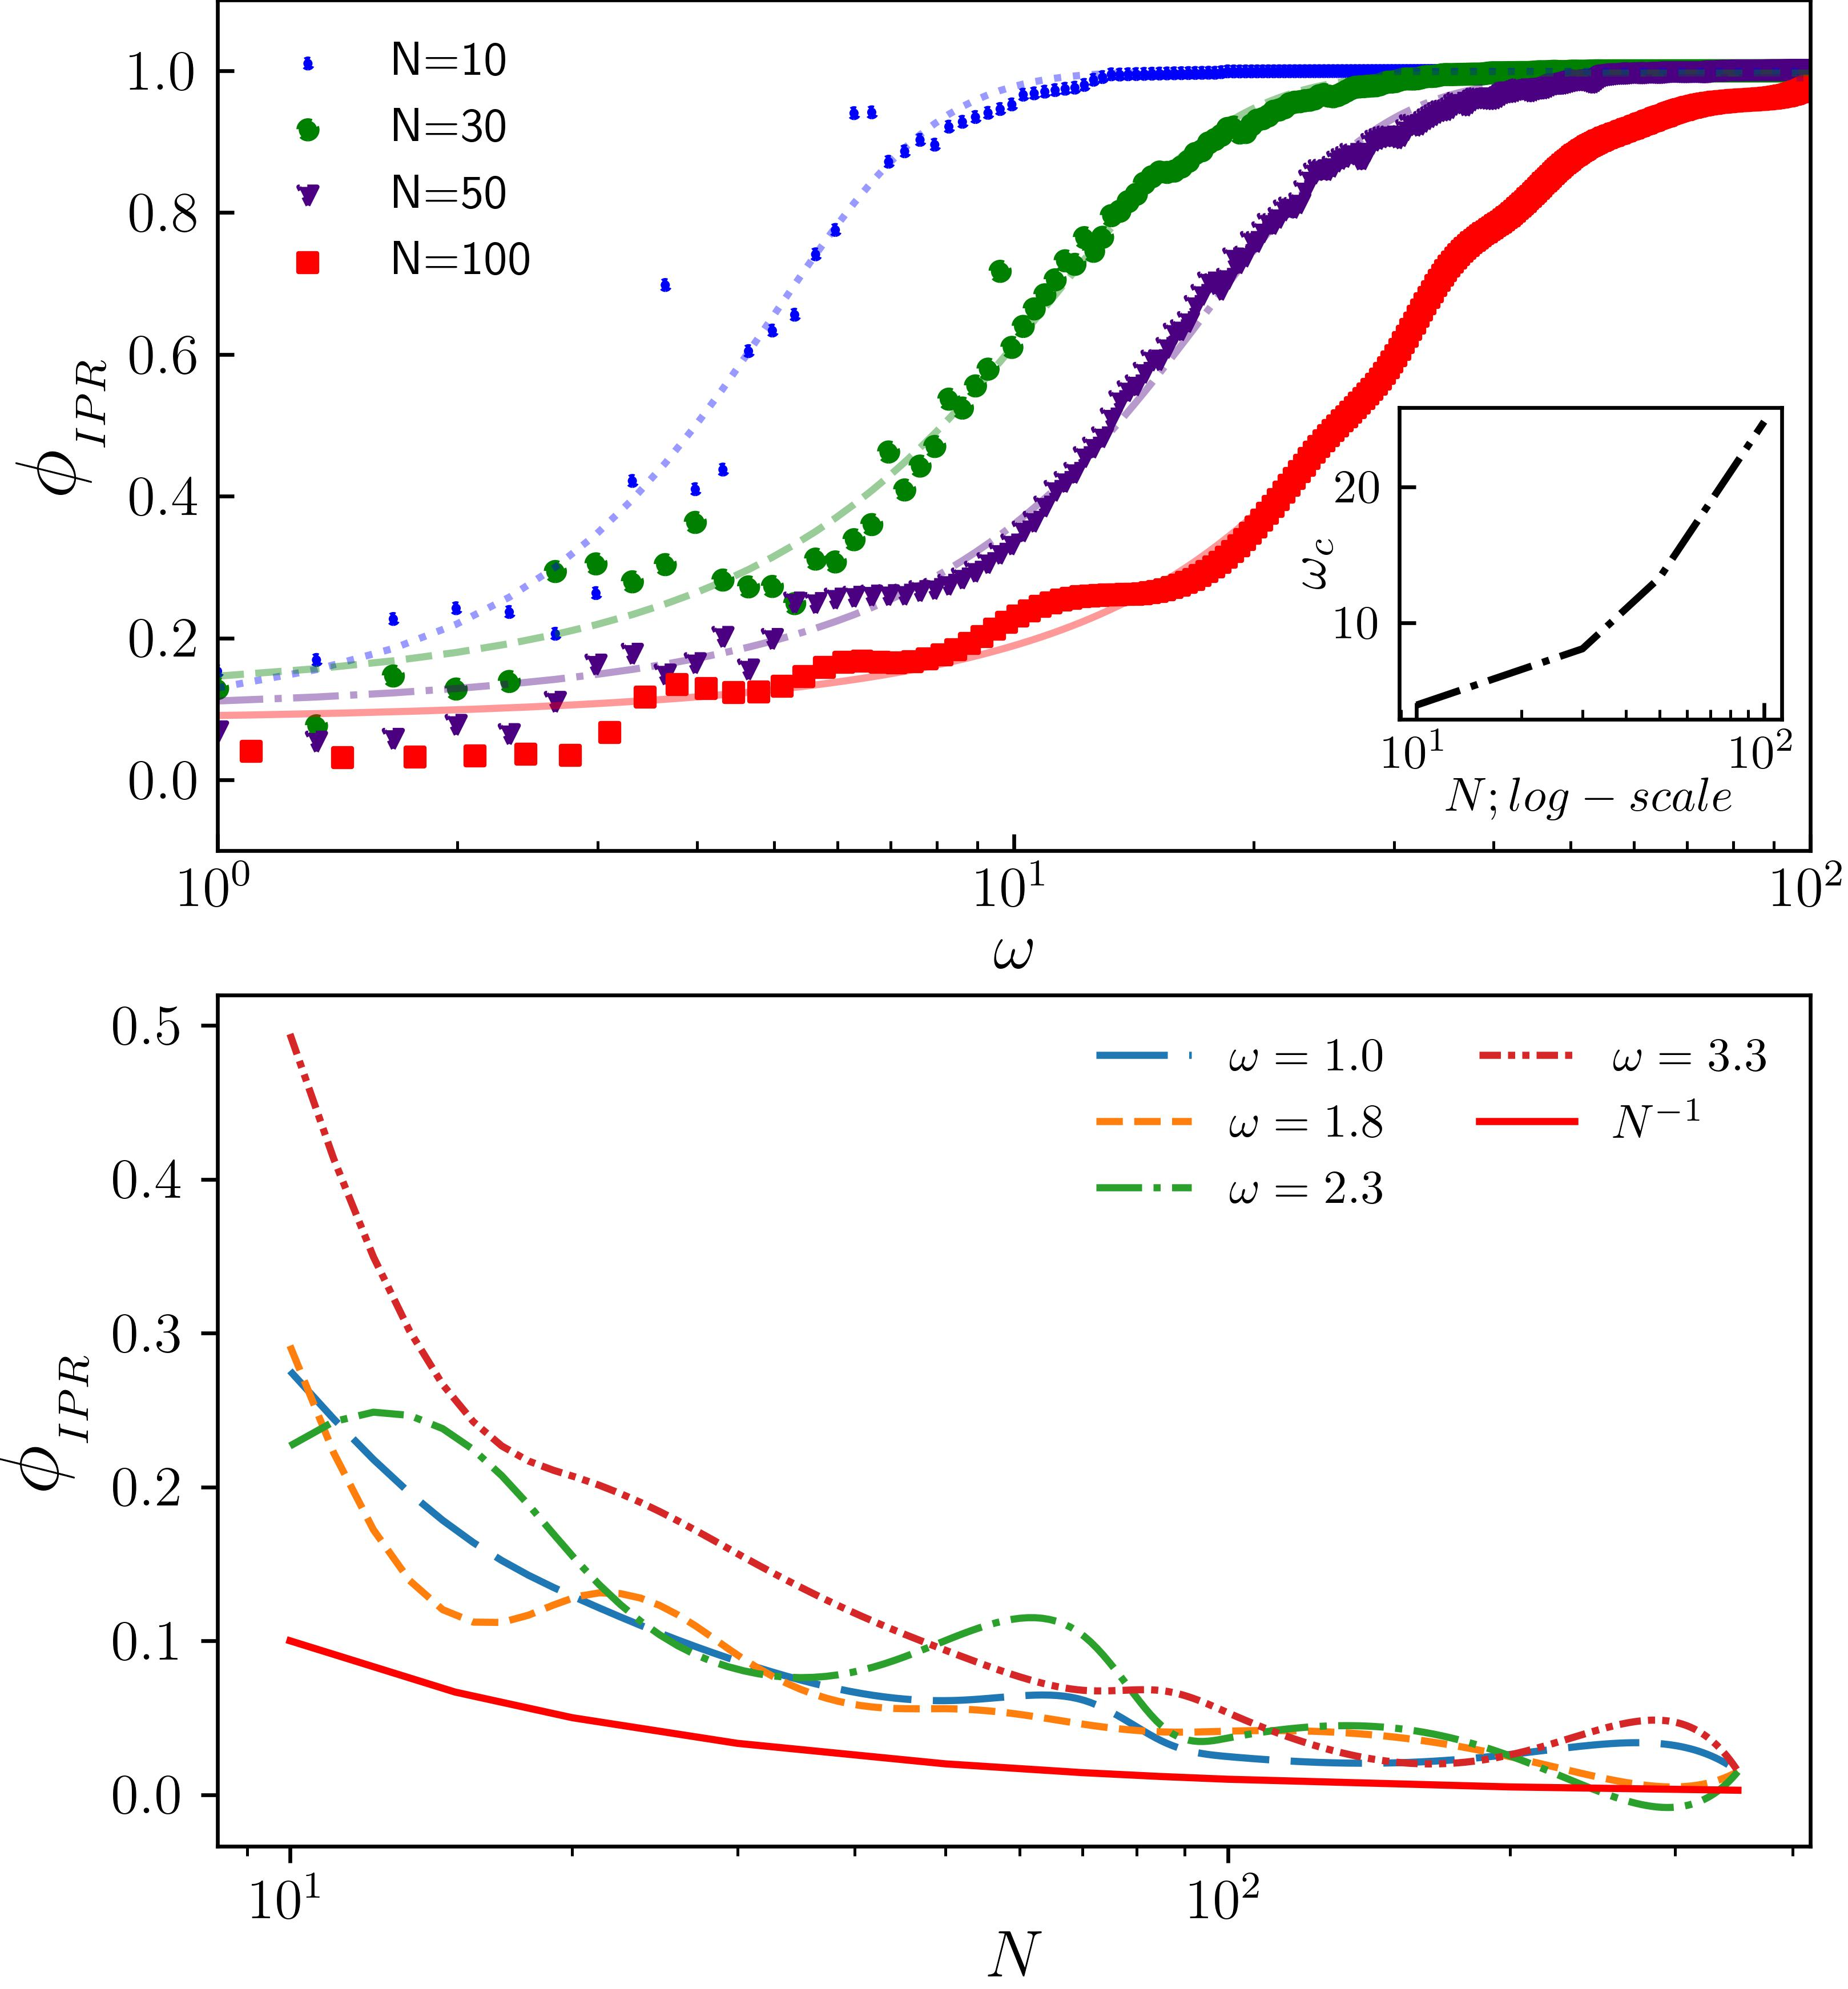
\includegraphics[height =9.0cm]{phase_crossover_LMG.jpeg}
		\caption{The plotting of the Inverse Participation Ratio (IPR) at Bessel's first root with first kind $J_0\Big(\frac{4h}{\omega}\Big)$ for varying drive amplitudes and frequencies in a spin array of LMG type, for different spin sizes $N = 10,30,50,100$. The adiabatic increase of the drive frequency is observed in the range of O(1) to O(50) for varying system sizes of N = 10, 30, 50, and 100. The study reveals that the IPR exhibits a decrease in magnitude at low frequencies, followed by an increase to unity at high frequencies, across various system sizes (top panel).  The findings indicate that the system's inverse participation ratio (IPR) diminishes in proportion to N in low-frequency regions, thereby validating the distribution of the system's state participation, as demonstrated in the lower panel. The increase in IPR with respect to system frequency exhibits a consistently gradual trend until it reaches a high frequency where IPR is unity, which is contingent upon system parameters. The lower panel indicates that the IPR decreases proportionally with the system size, which can be attributed to the distribution of states at lower frequencies.}
		\label{fig:phase_transition}
	\end{figure}

	The numerical evolution of the system is carried out using the exact Hamiltonian for a duration of 500 time periods. The average of the Hamiltonian, denoted as $\expval{\hat{H}}$, is then computed to determine the energy spreading through the standard deviation. The thermal conditions necessitate minimal fluctuations in energy distribution, as the spread of states leads to a limited standard deviation\cite{reimann_symmetry-prohibited_2021}. As a result, finite standard deviation arises in athermal regions. A graph depicting the standard deviation of the energy expectation value is presented for a system Hamiltonian adiabatically varied with drive frequency. The standard deviation of the Hamiltonian, denoted as $\expval{H}_{std}$, exhibits a small value for frequencies up to approximately $\omega \sim 5.0$. Subsequently, there is an increase in  that follows a linear pattern as the frequency increases further $\expval{H}_{std}$ in FIG\ref{fig:havg_std}. A thermal region is observed at a lower frequency, while an athermal region is detected at a higher frequency.
	
	\begin{figure}[!ht]
		\centering
		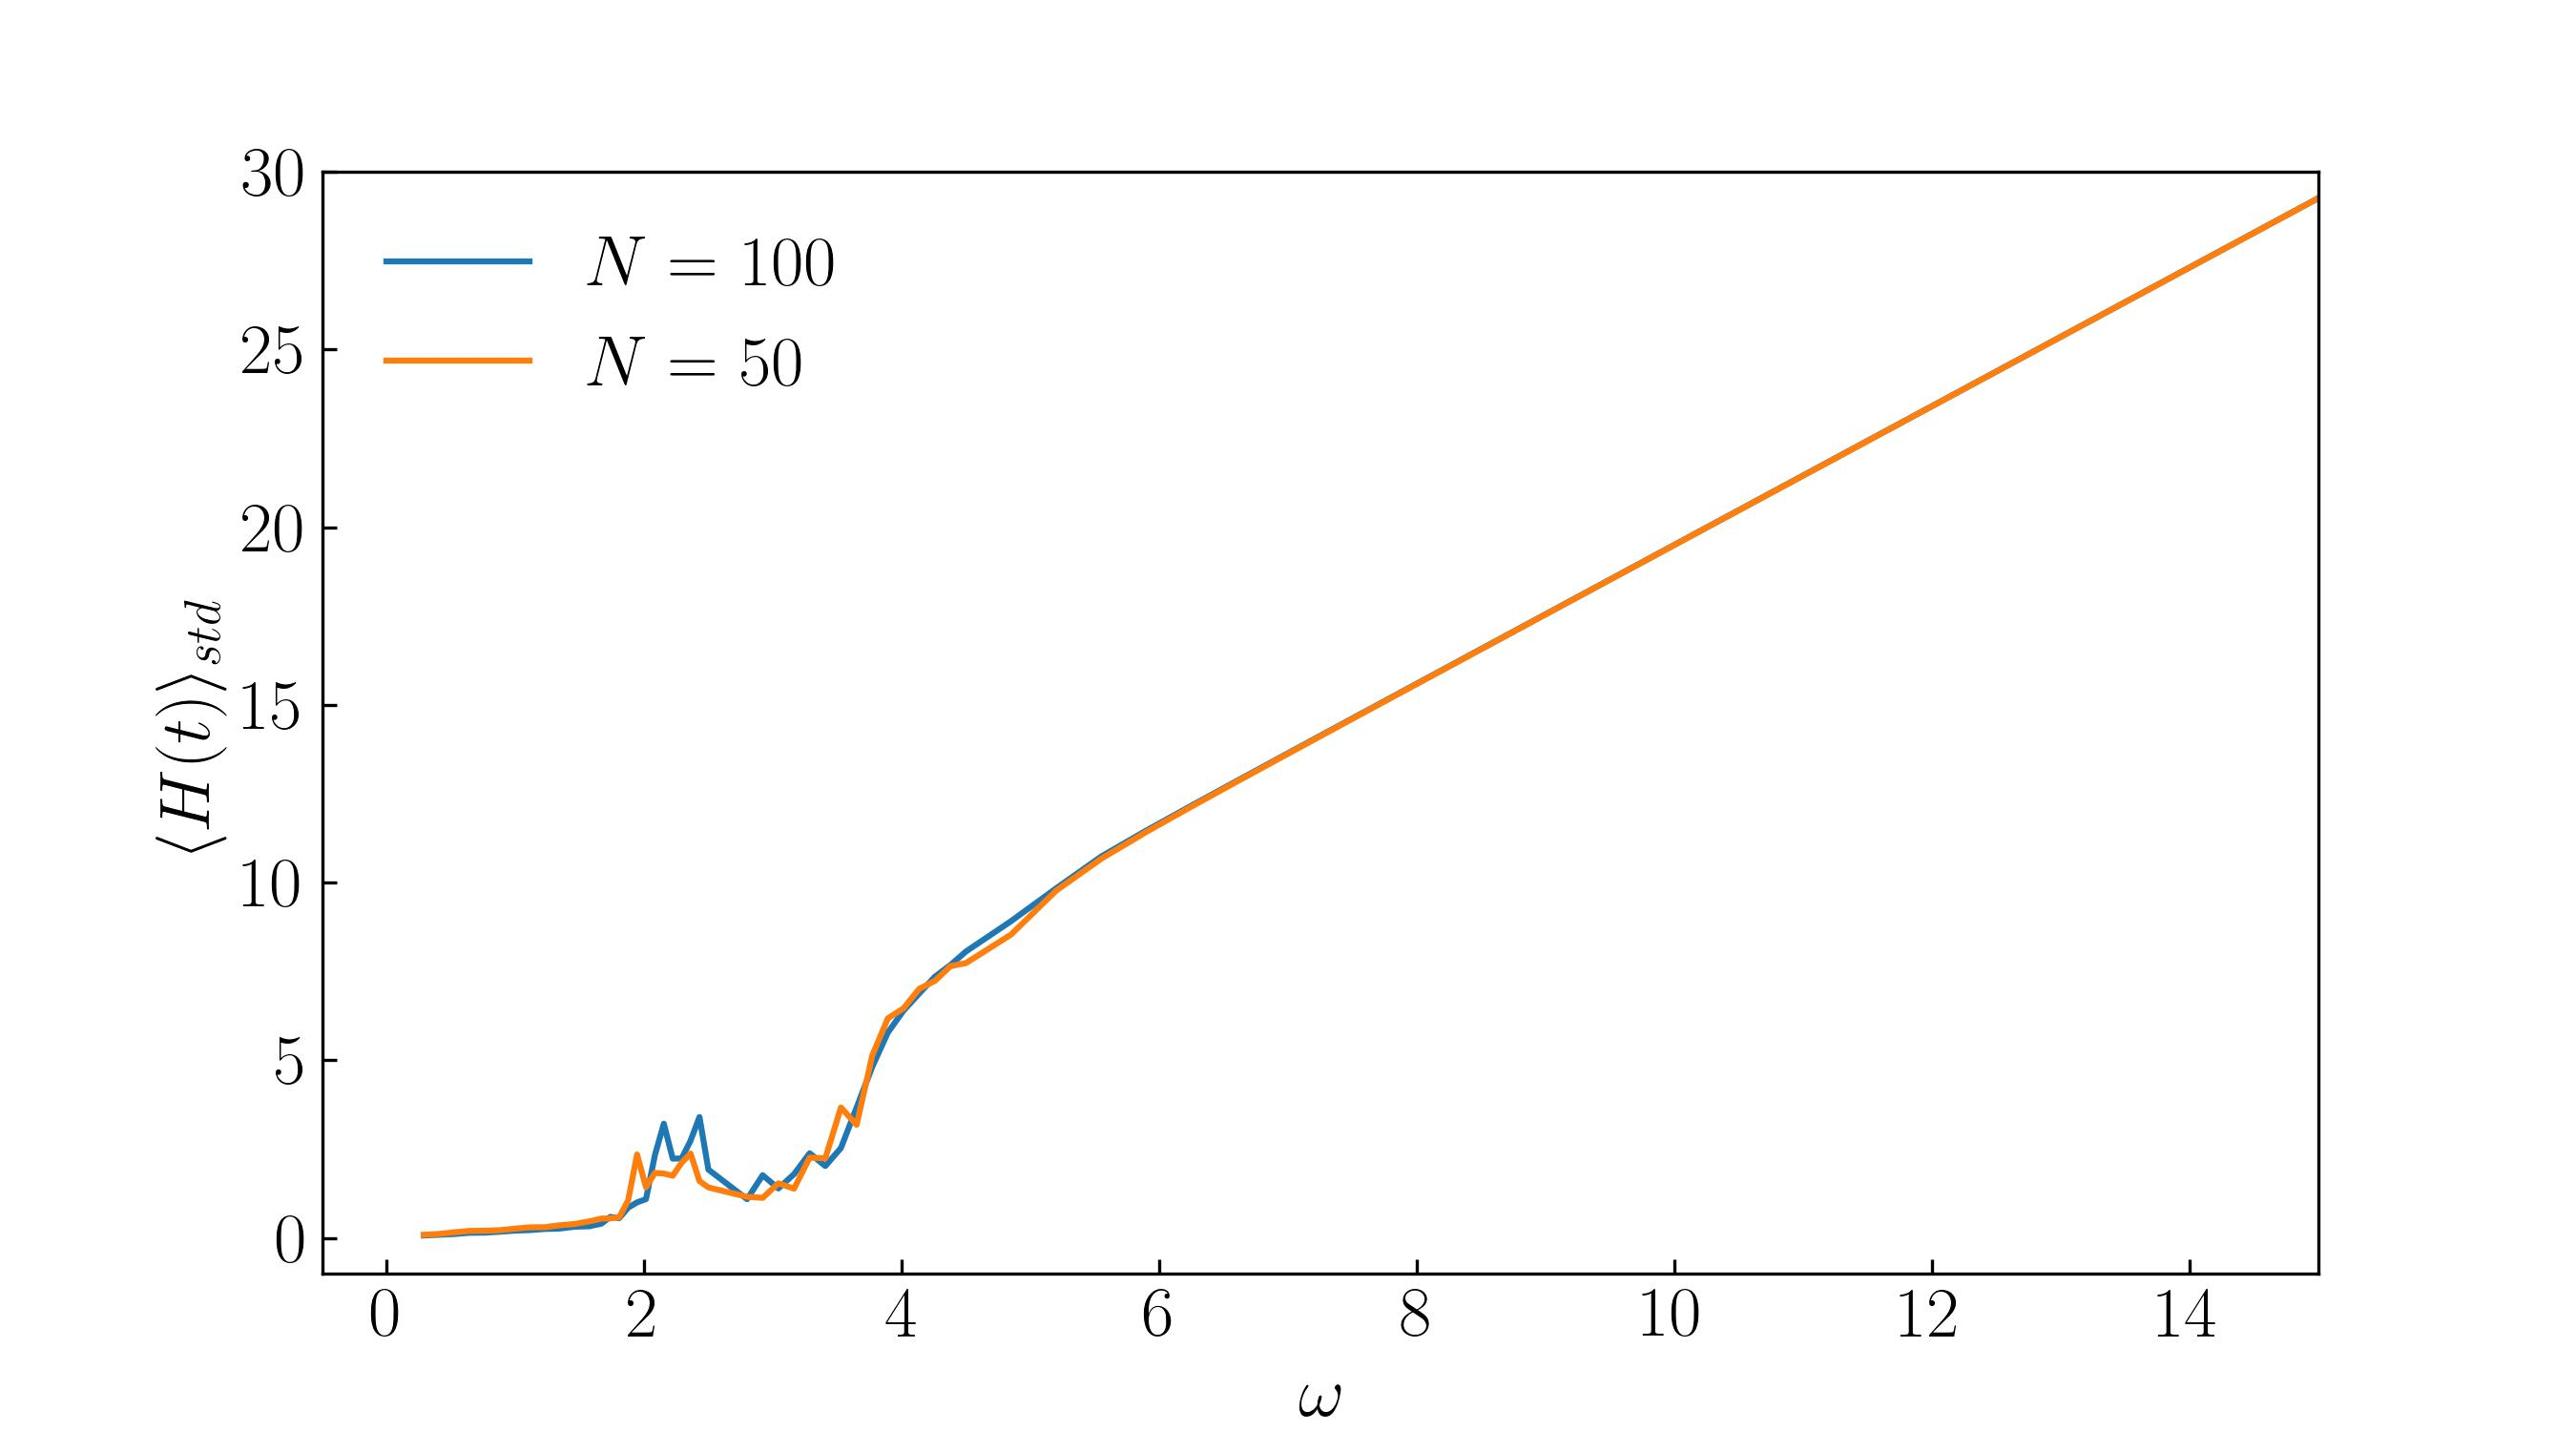
\includegraphics[width = 9.0cm]{hbar_std.jpg}
		\caption{The standard deviation of the mean value of H, denoted by $\expval{H}_{std}$, has been calculated over a span of 500 time periods. A singularity has been identified at approximately $\omega = 5.0$. The standard expectation value of the Hamiltonian, denoted as $\expval{H}_{std}$, exhibits a diminutive magnitude below the singularity, while a linear and gradual augmentation is observed at higher frequencies. A small standard deviation indicates the presence of a thermal region, whereas a larger finite standard deviation suggests the existence of a regular athermal region.}
		\label{fig:havg_std}
	\end{figure}
	
	
	\section{\label{sec:level6}Observations and Discussion}
	
	The quantum many-body localization in the Ising model is observed at high drive frequency and corresponding high drive amplitude, where the localization points are determined by setting $J_0(2h/{\omega}\big)=0$ for both exact and Rotated wave simulations. The delocalization away from the localization points is relatively weak. The integrability of the Ising model allows for localization to be observed at low values of $\omega$, despite the breakdown of the rotating wave approximation. Analytical methods beyond the adiabatic limit are intricate. The LMG model exhibits distinct localization at localization points, which are determined by the condition $J_0(4h/\omega)=0$, in both the exact and Rotated Wave simulations. However, there is some degree of delocalization observed beyond these points, albeit weak. The non-integrability of the LMG model and the established onset of chaos in the thermodynamic limit at low $\omega$ lead to a near-complete delocalization in the Inverse Participation Ratio (IPR) of the Floquet states at small $\omega$. 
	
	Consequently, we adiabatically varied $\omega, h$ in the LMG model, under the constraint that $\eta=4h/\omega$ was held at a root of $J_0(\eta)$. There, we observed a crossover or phase change from nearly fully thermal to completely localised behaviour (see FIG.\ref{fig:phase_transition}).
	Even if the limitation is relaxed, the macroscopic behaviour changes from thermal to athermal.
	At low frequencies, IPR is observed to decrease with increasing system size N, and when N is big, i.e., $\rightarrow{} \infty$, IPR appears to evaporate, resulting in a fully thermalized state at $\eta=4h/\omega$.
	This is in contrast to the Ising model, which lacks such a change in phase. Thus, the incorporation of long-range interactions appears to trigger a change in phase from the thermal phase to the localised phase, a property that will prove useful in the design of MBL engines. 
	
	\section{\label{sec:level7}Conclusion and Outlook}
	
	The study delved into the onset of Dynamical Many-Body Localization in the Lipkin-Glick-Meshkov spin model, specifically in regularly driven long-range spins, serving as a paradigmatic illustration. The parametrization of many-body localization is based on the Inverse Participation Ratio of the Floquet eigenstates.The present study conducted a numerical comparison between the inverse participation ratio (IPR) of the LMG model and the transverse field Ising model (TFIM) at both low and high drive frequencies. The present study involved an examination of the phase space dynamics of the LMG model. Specifically, we sought to analyze the emergence of thermal behavior at low frequencies and localization at high frequencies, as well as the appearance of additional approximately conserved quantities in the high-frequency regime for both models.
	
	\emph{Conclusion}: Long-range spins exhibit strong localization in spin-coordinate space for the LMG model when the drive frequency is $\omega \gg J$, where $J$ represents the spin exchange energy. The localization of the LMG model occurs at specific resonances of the drive frequency $\omega$ and amplitude $h$, where $J_0(4h/\omega)=0$. The TFIM case has shown comparable localization (in momentum space) at resonances determined by $J_0(2h/\omega)=0$. However, the mechanism differs in long-range systems as a distinct observable $(S_x)^2$ is conserved in the LMG case, where $\mathbf{S}$ represents the total spin. Upon the removal of accidental degeneracy through the application of a DC transverse field in the form of $\sim \hat{S_x}$, the eigenstates can be mapped into a coordinate representation, leading to a robust spatial localization. The periodically driven LMG model exhibits a pronounced mobility edge when the frequency is gradually increased from $\omega \sim J$ to $\omega \gg J$ in an adiabatic manner. In the first region where frequency $\omega$ is small, the quantum system is expected to undergo thermalization at exceedingly high temperatures due to the attainment of dynamical chaos in classical dynamics.However, in the latter high frequency regime, the perpetual postponement occurs due to dynamical localization. The point of transition in mobility between these two regimes exhibits anomalous characteristics when analyzed in the context of thermodynamic principles, indicating a quantum change in phase which detected as $phase-crossover$ between them. The absence of thermal behavior in the low-frequency limit of the short-range transverse field Ising model (TFIM) can be attributed to the significant magnitude of the inverse participation ratio (IPR). The induction of Thermal and Localized states in long-range systems can be achieved through Floquet engineering, without the need for disorder.	
	
	\emph{Outlook}: 	
	A system characterized by high symmetry has been thoroughly examined in a pristine state. Thermalization takes place in all scenarios, alongside integrability-disrupting factors, such as disorder. However, akin to TFIM, the onset of thermalization in LMG can be postponed when the condition $\omega\gg J$ and $J_0(4h/\omega) = 0$ is satisfied. In systems possessing a Hamiltonian of the form given by equations~\ref{eq:curieweiss:ham} and~\ref{eq:jij}, the time-independent Schrödinger equation can be solved analytically for certain potentials. The intermediate spin-spin interaction power law limits have received less attention compared to the infinite and long-range limit. Further research can be conducted on this topic. The LMG spin configuration undergoes a phase cross-over due to the adiabatic increase in drive frequency. This suggests the possibility of a future MBL engine that can operate between the thermal and localized regimes, with a thermodynamic cycle. Additionally, there exist prospects for diabatic corrections. 
	
	
	{\it Acknowledgement:}
	One of the authors, MR would like to acknowledge The University of Burdwan for support via a state-funded fellowship, as well as for providing computational resources. AR acknowledges support from the University Grants Commission (UGC) of India, via BSR Startup Grant No. F.30-425/2018(BSR), as well as from the Science and Engineering Research Board (SERB) Core Research Grant No. CRG/20l8/004002.
	
	% The \nocite command causes all entries in a bibliography to be printed out
	% whether or not they are actually referenced in the text. This is appropriate
	% for the sample file to show the different styles of references, but authors
	% most likely will not want to use it.
	\nocite{*}
	
	\bibliography{main}% Produces the bibliography via BibTeX.
	
\end{document}
%
% ****** End of file apssamp.tex ******